\documentclass[14pt, table]{extarticle}
\usepackage{amsfonts}
\usepackage{amsmath}
\usepackage[utf8]{inputenc}
\usepackage[a4paper, total={7in, 10.5in}]{geometry}
\usepackage[table]{xcolor}
\usepackage{tgbonum}
\usepackage{float}
\usepackage{graphicx}
\graphicspath{ {./images/} }
\DeclareGraphicsExtensions{.png,.jpg}
\usepackage{caption}
\usepackage{tikz}
\usepackage{circuitikz}
\usepackage[T1]{fontenc}
\usetikzlibrary{quotes,angles}
\usetikzlibrary{arrows}
\usetikzlibrary{circuits.logic.US}
\usetikzlibrary{positioning}
\hyphenpenalty 5000
\usepackage{subfig}
\usepackage{array}

\title{\textbf{Sprawozdanie} \\ \Large{Ćwiczenie 5}}
\date{Data wykonania: 24 maja 2023}
\author{ \Large{Jan Kwinta, grupa 12} \\ \large{Prowadzący ćwiczenia: dr. Szymon Niedźwiedzki}}

\newcommand{\nl}{\vspace{0.5cm}}
\newcommand{\nz}{\vspace{1.5cm}}

\begin{document}
\maketitle

\paragraph{Wstęp \\}

Przedmiotem piątych laboratoriów z elektroniki były układy cyfrowe o większym stopniu złożoności niż na poprzednich zajęciach. Montowaliśmy układy synchroniczne — przerzutniki synchroniczne, liczniki binarne,  dzielniki częstotliwości i rejestry. Używaliśmy do ich budowy wiele różnych układów scalonych z serii 74: 7400 i 7410 (bramki NAND dwu-  i trzywejściowe), 7474 (przerzutnik jednozboczowy D), 7475 (D \textit{latch}), 7493  (przerzutnik JK) oraz 74164 i 74165 (rejestry). \\

Układy synchroniczne to takie układy sekwencyjne, których zmiana stanu wewnętrznego następuje wyłącznie w określonych chwilach. Chwile te wyznacza sygnał zegarowy (ang. \textit{clock}), czyli generowany przez osobny układ sygnał o kształcie prostokątnym o stałej częstotliwości i amplitudzie wachającej się pomiędzy logiczną prawdą a logicznym fałszem. \\

Do realizacji zadań używałem jako sygnału zegarowego fali prostokątnej generatora, którą ustawiałem na małą częstotliwość (w okolicach $0.5 \ Hz$), aby móc operować wejściami układów (impulsatorami na płytce UC-2) w różnych momentach okresu zegara. Amplituda sygnału wynosiła $5 \ V$pp. Wartości sygnału zawierały się pomiędzy $0 \ V$ a $5 \ V$, co jest równoważne sygnałom logicznym fałsz i prawda na płytkach UC-2.

\newpage
\paragraph{Ćwiczenie 5.1 \\}
Zmontowanie synchronicznego przerzutnika RS korzystając z układów scalonych 7400 i 7410. Zbadanie działania przerzutnika oraz własności wejść \textit{a, b, c} i \textit{d}.

\begin{center}
\begin{tikzpicture}[circuit logic US, scale=2]

	\node [nand gate, inputs=nnn] (nand1) at (0, 0) {};
	\node [nand gate, inputs=nnn] (nand2) at (0, -2) {};
	\node [nand gate, inputs=nnn] (nand3) at (3, 0) {};
	\node [nand gate, inputs=nnn] (nand4) at (3, -2) {};

	\draw (nand1.input 1) -- node[at end, left]{\textit{a}} ++(left: 1);
	\draw (nand2.input 3) -- node[at end, left]{\textit{b}} ++(left: 1);
	\draw (nand3.input 1) -- node[at end, left]{\textit{c}} ++(left: 1);
	\draw (nand4.input 3) -- node[at end, left]{\textit{d}} ++(left: 1);

	\node (CLK) at (-1.8, -1) {CLK};

	\draw (CLK.east) -- node [at end, circle, fill, inner sep=1.3pt]{}(-1, -1);
	\draw (-1, -1) |- (nand1.input 3);
	\draw (-1, -1) |- (nand2.input 1);

	\draw (nand1.output) -| (nand3.input 2);
	\draw (nand2.output) -| (nand4.input 2);

	\draw (nand3.output) -- node (q1) [at end, circle, fill, inner sep=1.3pt]{} ++(right: 0.5);
	\draw (nand4.output) -- node (q2) [at end, circle, fill, inner sep=1.3pt]{} ++(right: 0.5);

	\draw (q1) -- node[at end, right]{$Q$} ++(right: 1);
	\draw (q2) -- node[at end, right]{$\overline{Q}$} ++(right: 1);

	\draw (q1) -- ++(down: 0.4) -- (2, -1.5) |- (nand4.input 1);
	\draw (q2) -- ++(up: 0.4) -- (2, -0.5) |- (nand3.input 3);

\end{tikzpicture}
\end{center}

Zmontowałem układ na płytce UC-2 według powyższego schematu, korzystając z bramek NAND: dwuwejściowych (7400) i trzywejściowych (7410). Układ ten posiada pięć wejść i dwa wyjścia. Pod wejście zegarowe (CLK) podłączyłem sygnał o częstotliwośći $0.1 \ Hz$ z generatora. Wejścia \textit{a} oraz \textit{b} połączyłem z wyjściami $Q$ impulsatorów na płytce. Na wejścia \textit{c} oraz \textit{d} podawałem stan logiczny prawda i fałsz spinając je odpowiednio do $+5 \ V$ przez opornik $1 \ k \Omega$ i do $0 \ V$ przez opornik $390 \ \Omega$. Wyjście $Q$ przerzutnika podłączyłem do próbnika stanów logicznych. \\

Z zegarem, zmieniając stany wejść \textit{c} i \textit{d} oraz operując impulsatorami zmierzyłem stan wyjścia $Q$ przy wszystkich różnych stanach wejść \textit{a, b, c, d} i CLK. Nagrania z pomiarów znajdują się w filmikach MP4 w pliku 
\texttt{Sprawozdanie-cwiczenie5-Jan-Kwinta-Zalacznik1.zip}. Na filmikach taktowanie zegara pokazuje skrajnie prawa dioda na płytce. \\

Wyniki pomiarów przedstawiłem w czterech tabelach zamieszczonych poniżej. Litera \textit{p} oznacza stan pamiętania.

\begin{table}[H]
\begin{minipage}{.5\linewidth}
\centering
\begin{tabular} { | c | c | c | c | c | c | c |}
\multicolumn{7}{ c }{\textit{c} = 0 \ \textit{d} = 0} \\
\hline
\hline
\multicolumn{3}{| c |}{CLK = 1} & {} & \multicolumn{3}{ c |}{CLK = 0} \\
\hline
\hline
\textit{a} & \textit{b} & $Q$ & {} & \textit{a} & \textit{b} & $Q$ \\
\hline
0 & 0 & 1 & {} & 0 & 0 & 1\\
\hline
0 & 1 & 1 & {} & 0 & 1 & 1\\
\hline
1 & 0 & 1 & {} & 1 & 0 & 1\\
\hline
1 & 1 & 1 & {} & 1 & 1 & 1\\
\hline
\end{tabular}

\end{minipage}%
\begin{minipage}{.5\linewidth}
\centering

\begin{tabular} { | c | c | c | c | c | c | c |}
\multicolumn{7}{ c }{\textit{c} = 0 \ \textit{d} = 1} \\
\hline
\hline
\multicolumn{3}{| c |}{CLK = 1} & {} & \multicolumn{3}{ c |}{CLK = 0} \\
\hline
\hline
\textit{a} & \textit{b} & $Q$ & {} & \textit{a} & \textit{b} & $Q$ \\
\hline
0 & 0 & 1 & {} & 0 & 0 & 1\\
\hline
0 & 1 & 1 & {} & 0 & 1 & 1\\
\hline
1 & 0 & 1 & {} & 1 & 0 & 1\\
\hline
1 & 1 & 1 & {} & 1 & 1 & 1\\
\hline
\end{tabular}
\end{minipage}
\end{table}

\begin{table} [H]
\begin{minipage}{.5\linewidth}
\centering
\begin{tabular} { | c | c | c | c | c | c | c |}
\multicolumn{7}{ c }{\textit{c} = 1 \ \textit{d} = 0} \\
\hline
\hline
\multicolumn{3}{| c |}{CLK = 1} & {} & \multicolumn{3}{ c |}{CLK = 0} \\
\hline
\hline
\textit{a} & \textit{b} & $Q$ & {} & \textit{a} & \textit{b} & $Q$ \\
\hline
0 & 0 & 0 & {} & 0 & 0 & 0\\
\hline
0 & 1 & 0 & {} & 0 & 1 & 0\\
\hline
1 & 0 & 1 & {} & 1 & 0 & 0\\
\hline
1 & 1 & 1 & {} & 1 & 1 & 0\\
\hline
\end{tabular}

\end{minipage}%
\begin{minipage}{.5\linewidth}
\centering

\begin{tabular} { | c | c | c | c | c | c | c |}
\multicolumn{7}{ c }{\textit{c} = 1 \ \textit{d} = 1} \\
\hline
\hline
\multicolumn{3}{| c |}{CLK = 1} & {} & \multicolumn{3}{ c |}{CLK = 0} \\
\hline
\hline
\textit{a} & \textit{b} & $Q$ & {} & \textit{a} & \textit{b} & $Q$ \\
\hline
0 & 0 & \textit{p} & {} & 0 & 0 & \textit{p}\\
\hline
0 & 1 & 0 & {} & 0 & 1 & \textit{p}\\
\hline
1 & 0 & 1 & {} & 1 & 0 & \textit{p}\\
\hline
1 & 1 & - & {} & 1 & 1 & \textit{p}\\
\hline
\end{tabular}
\end{minipage}
\end{table}

Analizując stany wyjścia w zależności od stanów wejść jestem w stanie zaobserwować kilka faktów:

\begin{itemize}
	\item Gdy na wejście zegarowe podany jest sygnał niski (0) układ nie reaguje na zmiany stanów wejść \textit{a} i \textit{b}.
	\item Gdy na wejście \textit{c} podany jest stan logiczny 0 na wyjściu $Q$ przerzutnika jest stan logiczny 1 niezależnie od innych wejść, co czyni przerzutnik transparentnym w logice NAND.
	\item Gdy na obydwa wejścia \textit{c} i \textit{d} podany jest sygnał wysoki to przerzutnik zachowuje się tak jak zwykły synchroniczny przerzutnik RS.
\end{itemize}

Można z tych obserwacji wyciągnąć następujące wnioski: Po pierwsze — synchroniczny przerzutnik RS może zmieniać swój stan wewnętrzny tylko wtedy, gdy na wejściu zegarowym jest stan logicznej jedynki. Po drugie — podanie fałszu na wejścia \textit{c} i \textit{d} powoduje odjęcie funkcjonalności układowi. Spięcie razem tych wejść stworzyłoby wejście włączające, czyli tak zwane \textit{chip enable} lub \textit{chip select} oznaczane zazwyczaj jako CE albo CS, które pozwala na selektywne włączanie i wyłączanie rejestru. Gdy na wejście CE podany jest sygnał 1 to cały układ działa, zachowując się jak normalny przerzutnik. Gdy wyłączymy układ, czyli podamy na wejście CE sygnał 0, nasz przerzutnik staje się dla jakiegoś większego układu, którego może być częścią, transparentny, czyli podaje na swoje wejście 1 niezależnie od stanu zegara czy wejść \textit{a} oraz \textit{b}. \\

Wiele bardziej zaawansowanych komponentów elektronicznych: mikroprocesory, układy pamięci, itp. posiada wejście CE lub CS, co pozwala na wygodne ich wykorzystywanie w dużych układach i urządzeniach. Umożliwia to na przykład sterowanie jednemu procesorowi wieloma ukła- dami pamięci podłączonymi do jednej magistrali komunikacyjnej.

\newpage
\paragraph{Ćwiczenie 5.2 \\}

Zbadanie działania przerzutnika jednozboczowego D (układ scalony 7474), podając na odpowiednie wejścia sygnał zegara, sygnały z impulsatora lub spinając z $0 \ V$ albo $5 \ V$. \\

Układ przerzutnika D znajdującego się na układach 7474 można przedstawić schematycznie tak:

\begin{center}
\begin{circuitikz} [circuit logic US, scale=2]
	
	\ctikzset{multipoles/dipchip/pin spacing=0.5}
	\node [anchor=pin 1, dipchip, num pins=8, hide numbers, no topmark, external pins width=0, scale=2](d1){};

	\node [right] at (d1.bpin 1) {\textsl{CLK}};
	\node [right] at (d1.bpin 2) {\textsl{CLR}};
	\node [right] at (d1.bpin 3) {\textsl{PRE}};
	\node [right] at (d1.bpin 4) {\textsl{D}};
	\node [left] at (d1.bpin 8) {\textsl{Q}};
	\node [left] at (d1.bpin 5) {\textsl{\ctikztextnot{Q}}};

	\draw (d1.bpin 1) -- ++(left: 0.7);
	\draw (d1.bpin 2) -- ++(left: 0.7);
	\draw (d1.bpin 3) -- ++(left: 0.7);
	\draw (d1.bpin 4) -- ++(left: 0.7);
	\draw (d1.bpin 5) -- ++(right: 0.7);
	\draw (d1.bpin 8) -- ++(right: 0.7);

\end{circuitikz}
\end{center}

Przerzutnik ten posiada 4 wejścia i dwa wyjścia. Wejście zegarowe oznaczone jest CLK (\textit{clock}), wejście na dane — D (\textit{data}). Wejścia CLR i PRE to odpowiednio \textit{clear} oraz \textit{preset}. Z dokumentacji producenta możemy dowiedzieć się, że są to wejścia normalizowane do stanu wysokiego (czyli przy podaniu na obydwa sygnału prawdziwego układ 7474 jest operacyjny jako przerzutnik D). Podanie sygnału niskiego na wejście CLR "czyści" przerzutnik, czyli ustawia wyjście $Q$ na 0 niezależnie od wejść CLK i D. Podanie sygnału niskiego na wejście PRE "ustawia" przerzutnik, czyli ustawia wyjście $Q$ na 1 niezależnie od wejść CLK i D. Podanie na obydwa wejścia CLR i PRE sygnału 0 jest stanem zabronionym. \\

Aby zbadać układ przerzutnika podłączyłem obydwa wejścia PRE i CLR "na sztywno" pod sygnał wysoki. Do wejścia CLK podpiąłem sygnał z generatora (na zdjęciach stan zegara widać na skrajnie prawej żółtej diodzie). Jeden z impulsatorów przyłączyłem do wejścia D. Skonstruowałem układ jak na zdjęciach na kolejnej stronie. Następnie podłączyłem wejście CLR a potem wejście PRE pod drugi impulsator (niestety z tych badań nie mam zdjęć).

\newpage
\begin{figure}[H]
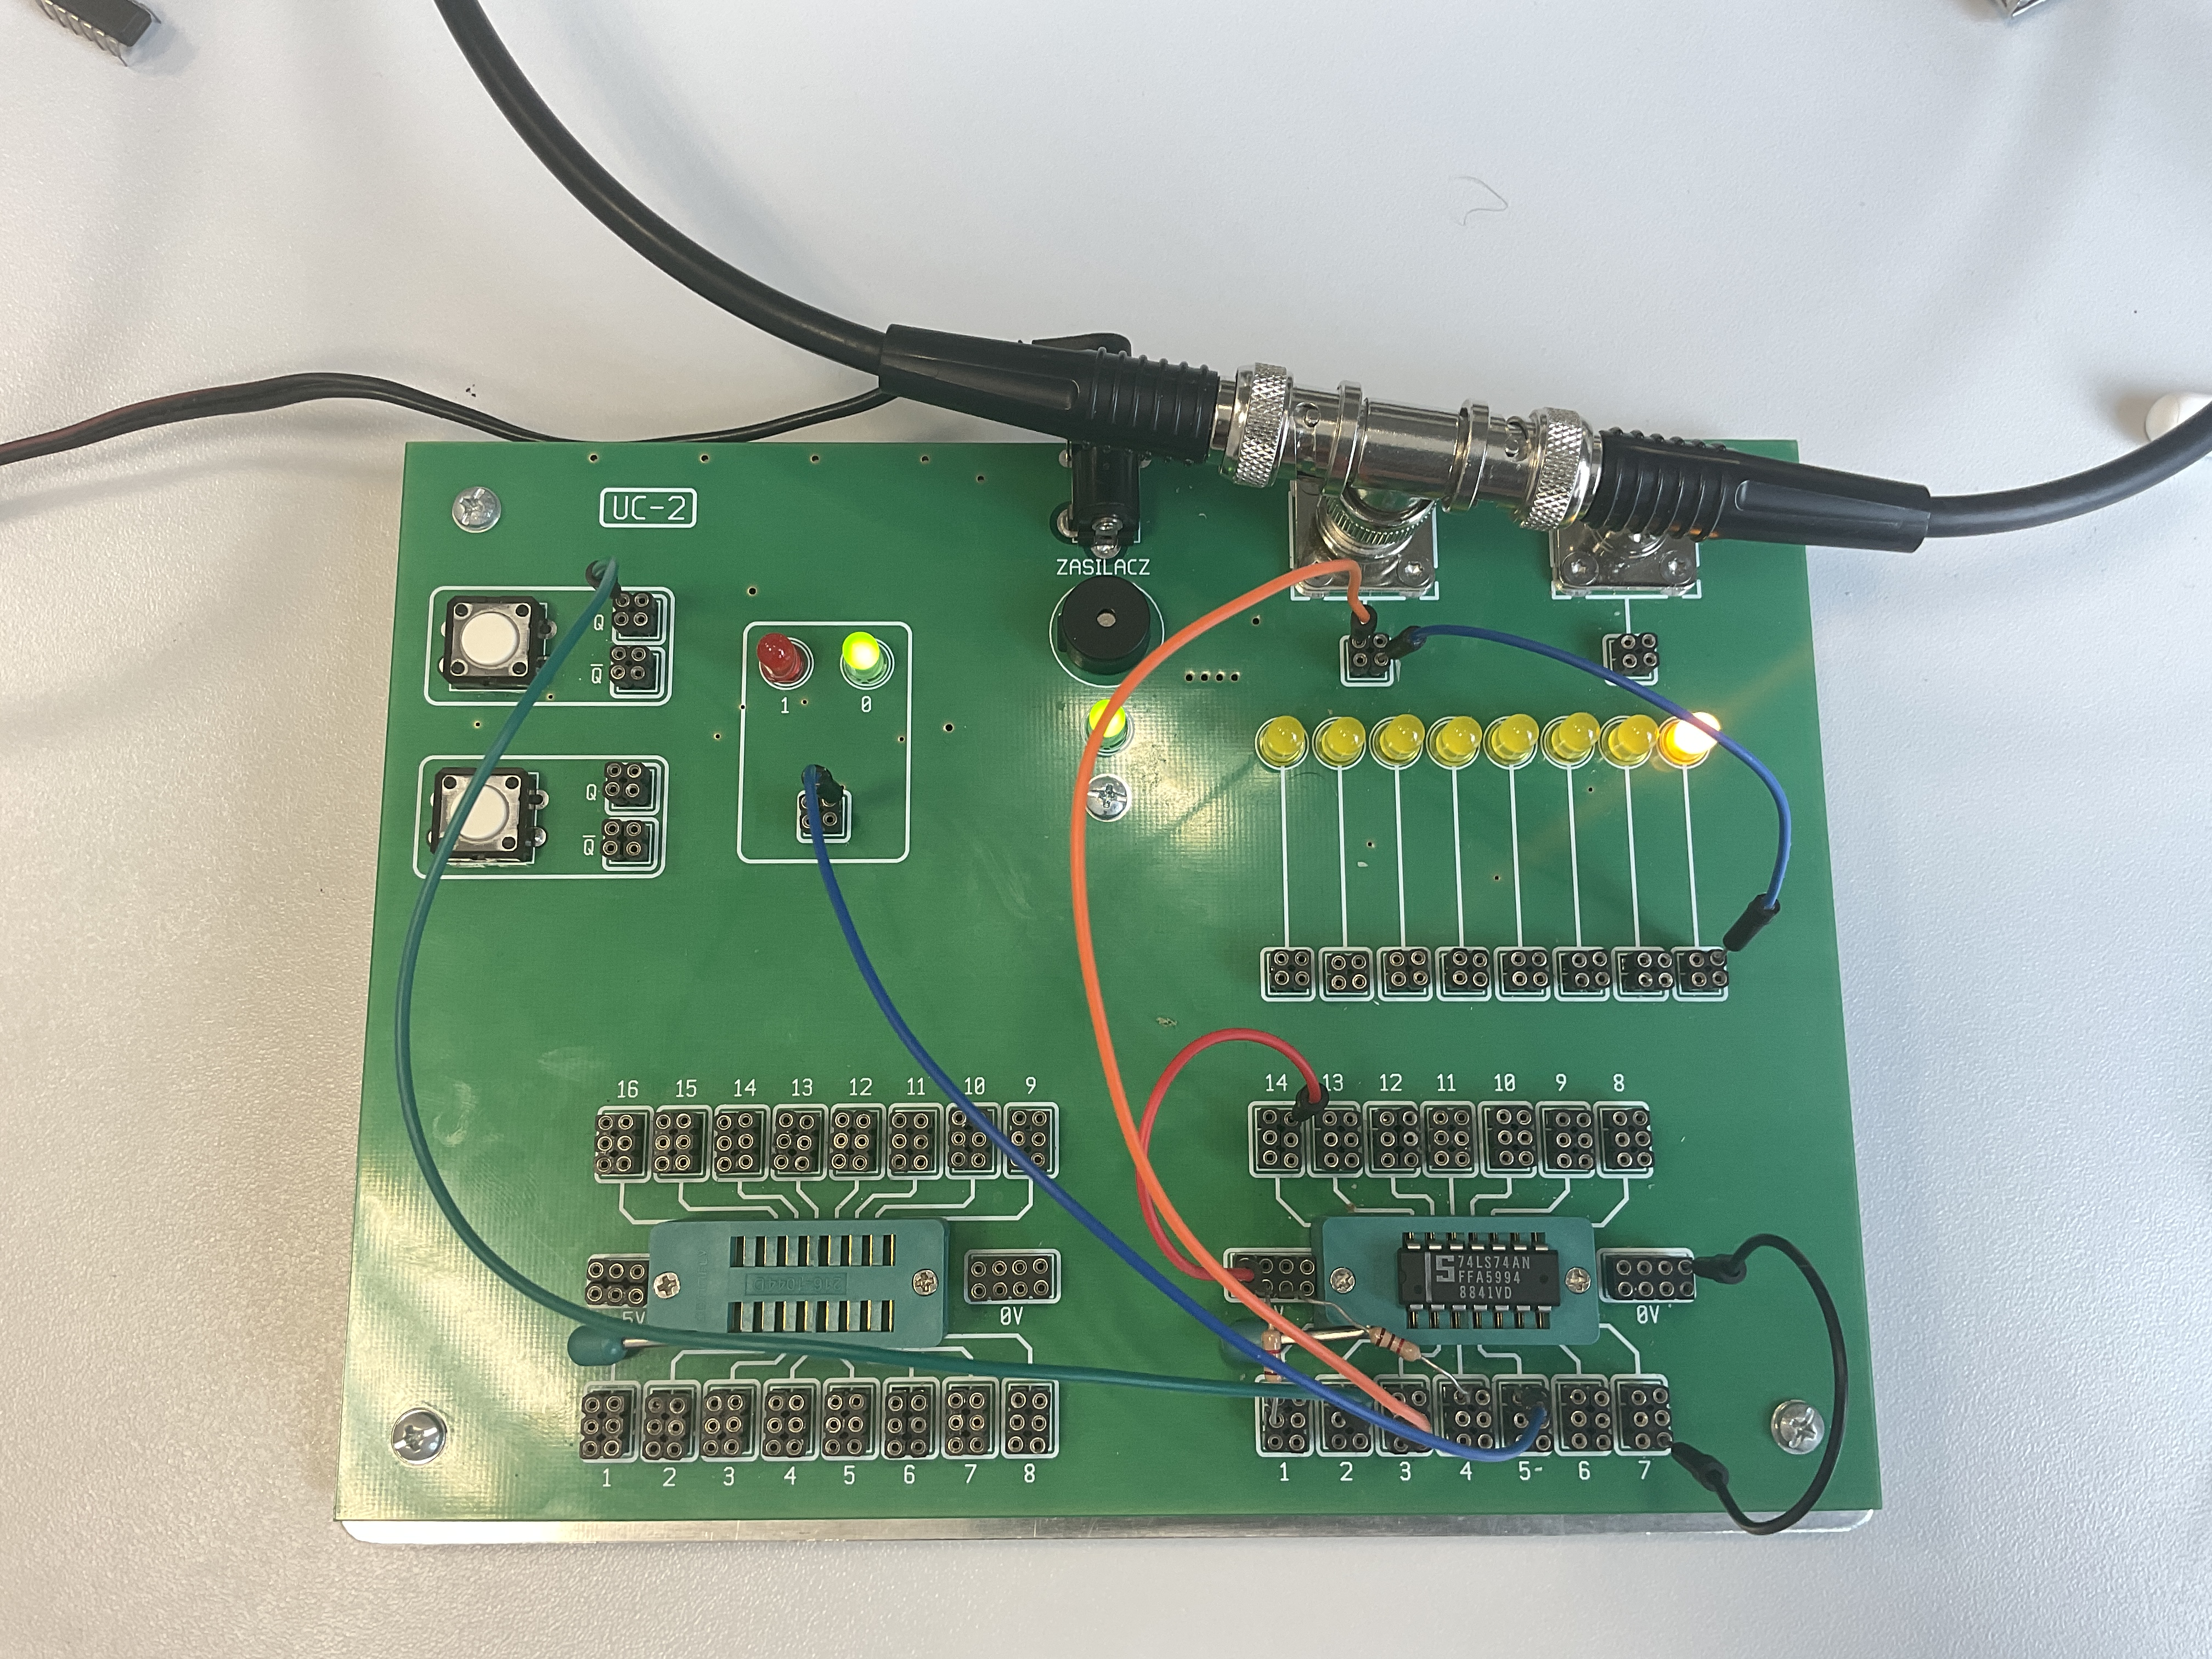
\includegraphics[width=7cm]{C0}
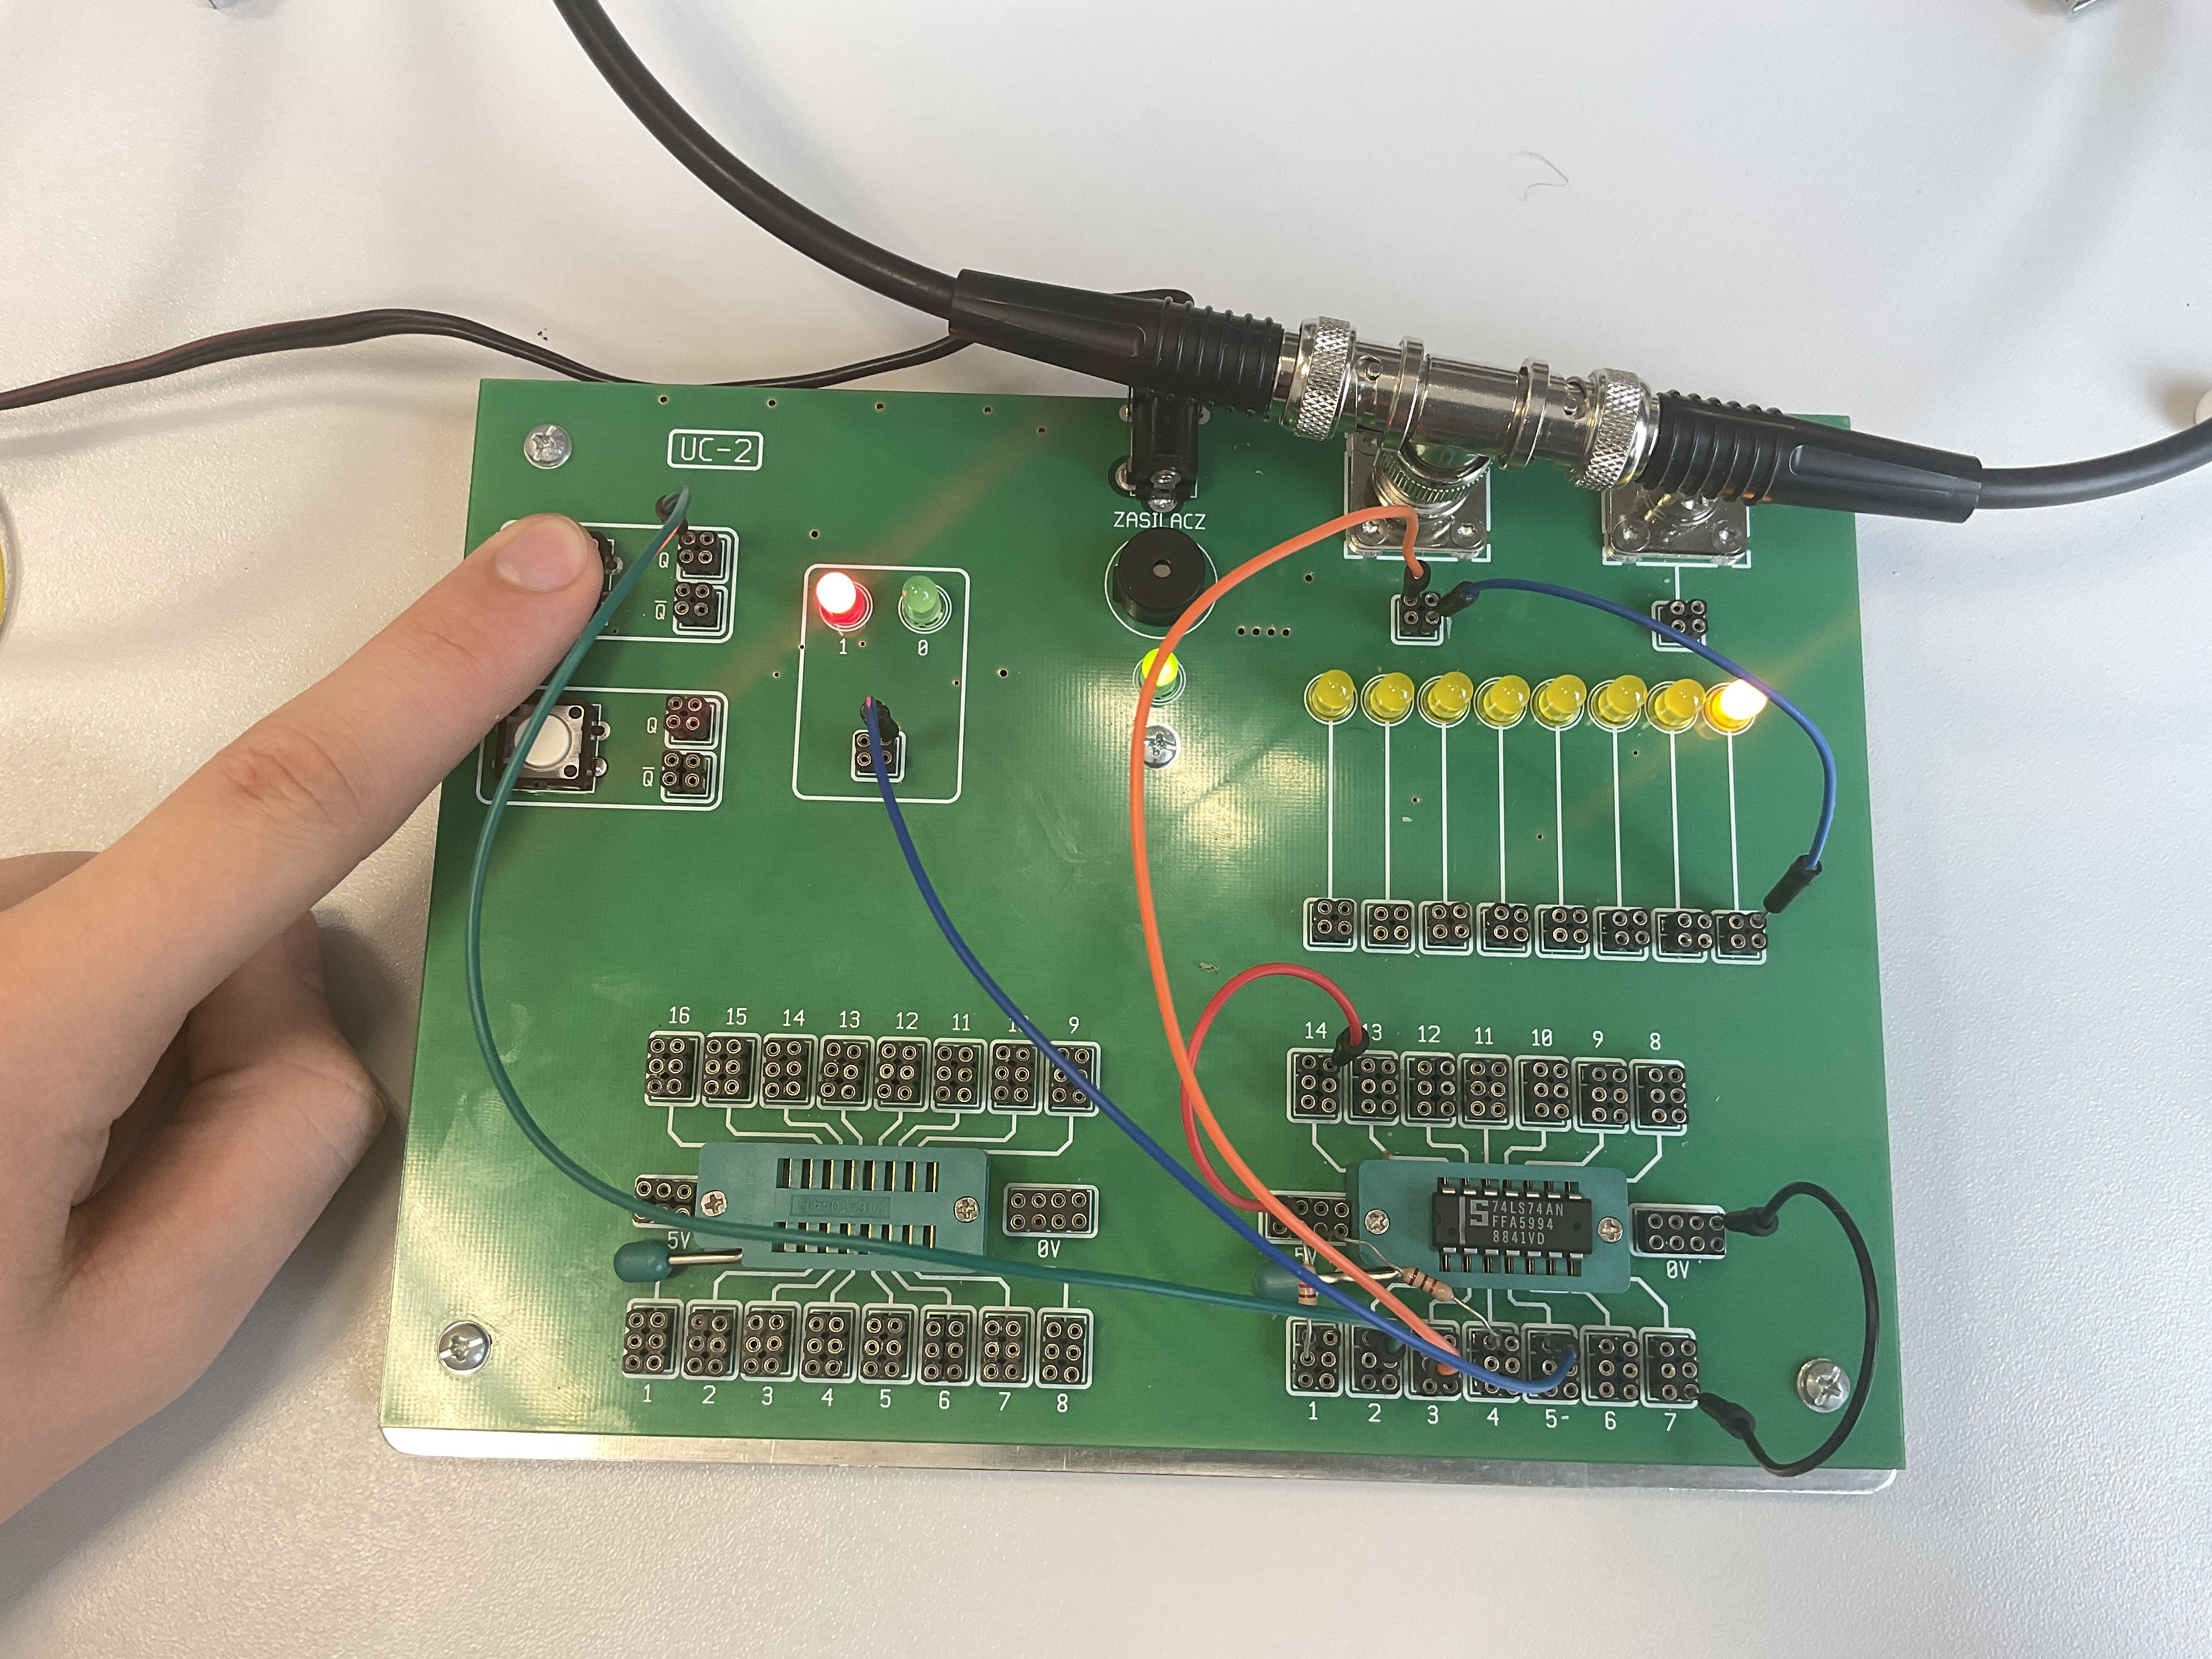
\includegraphics[width=7cm]{C1}
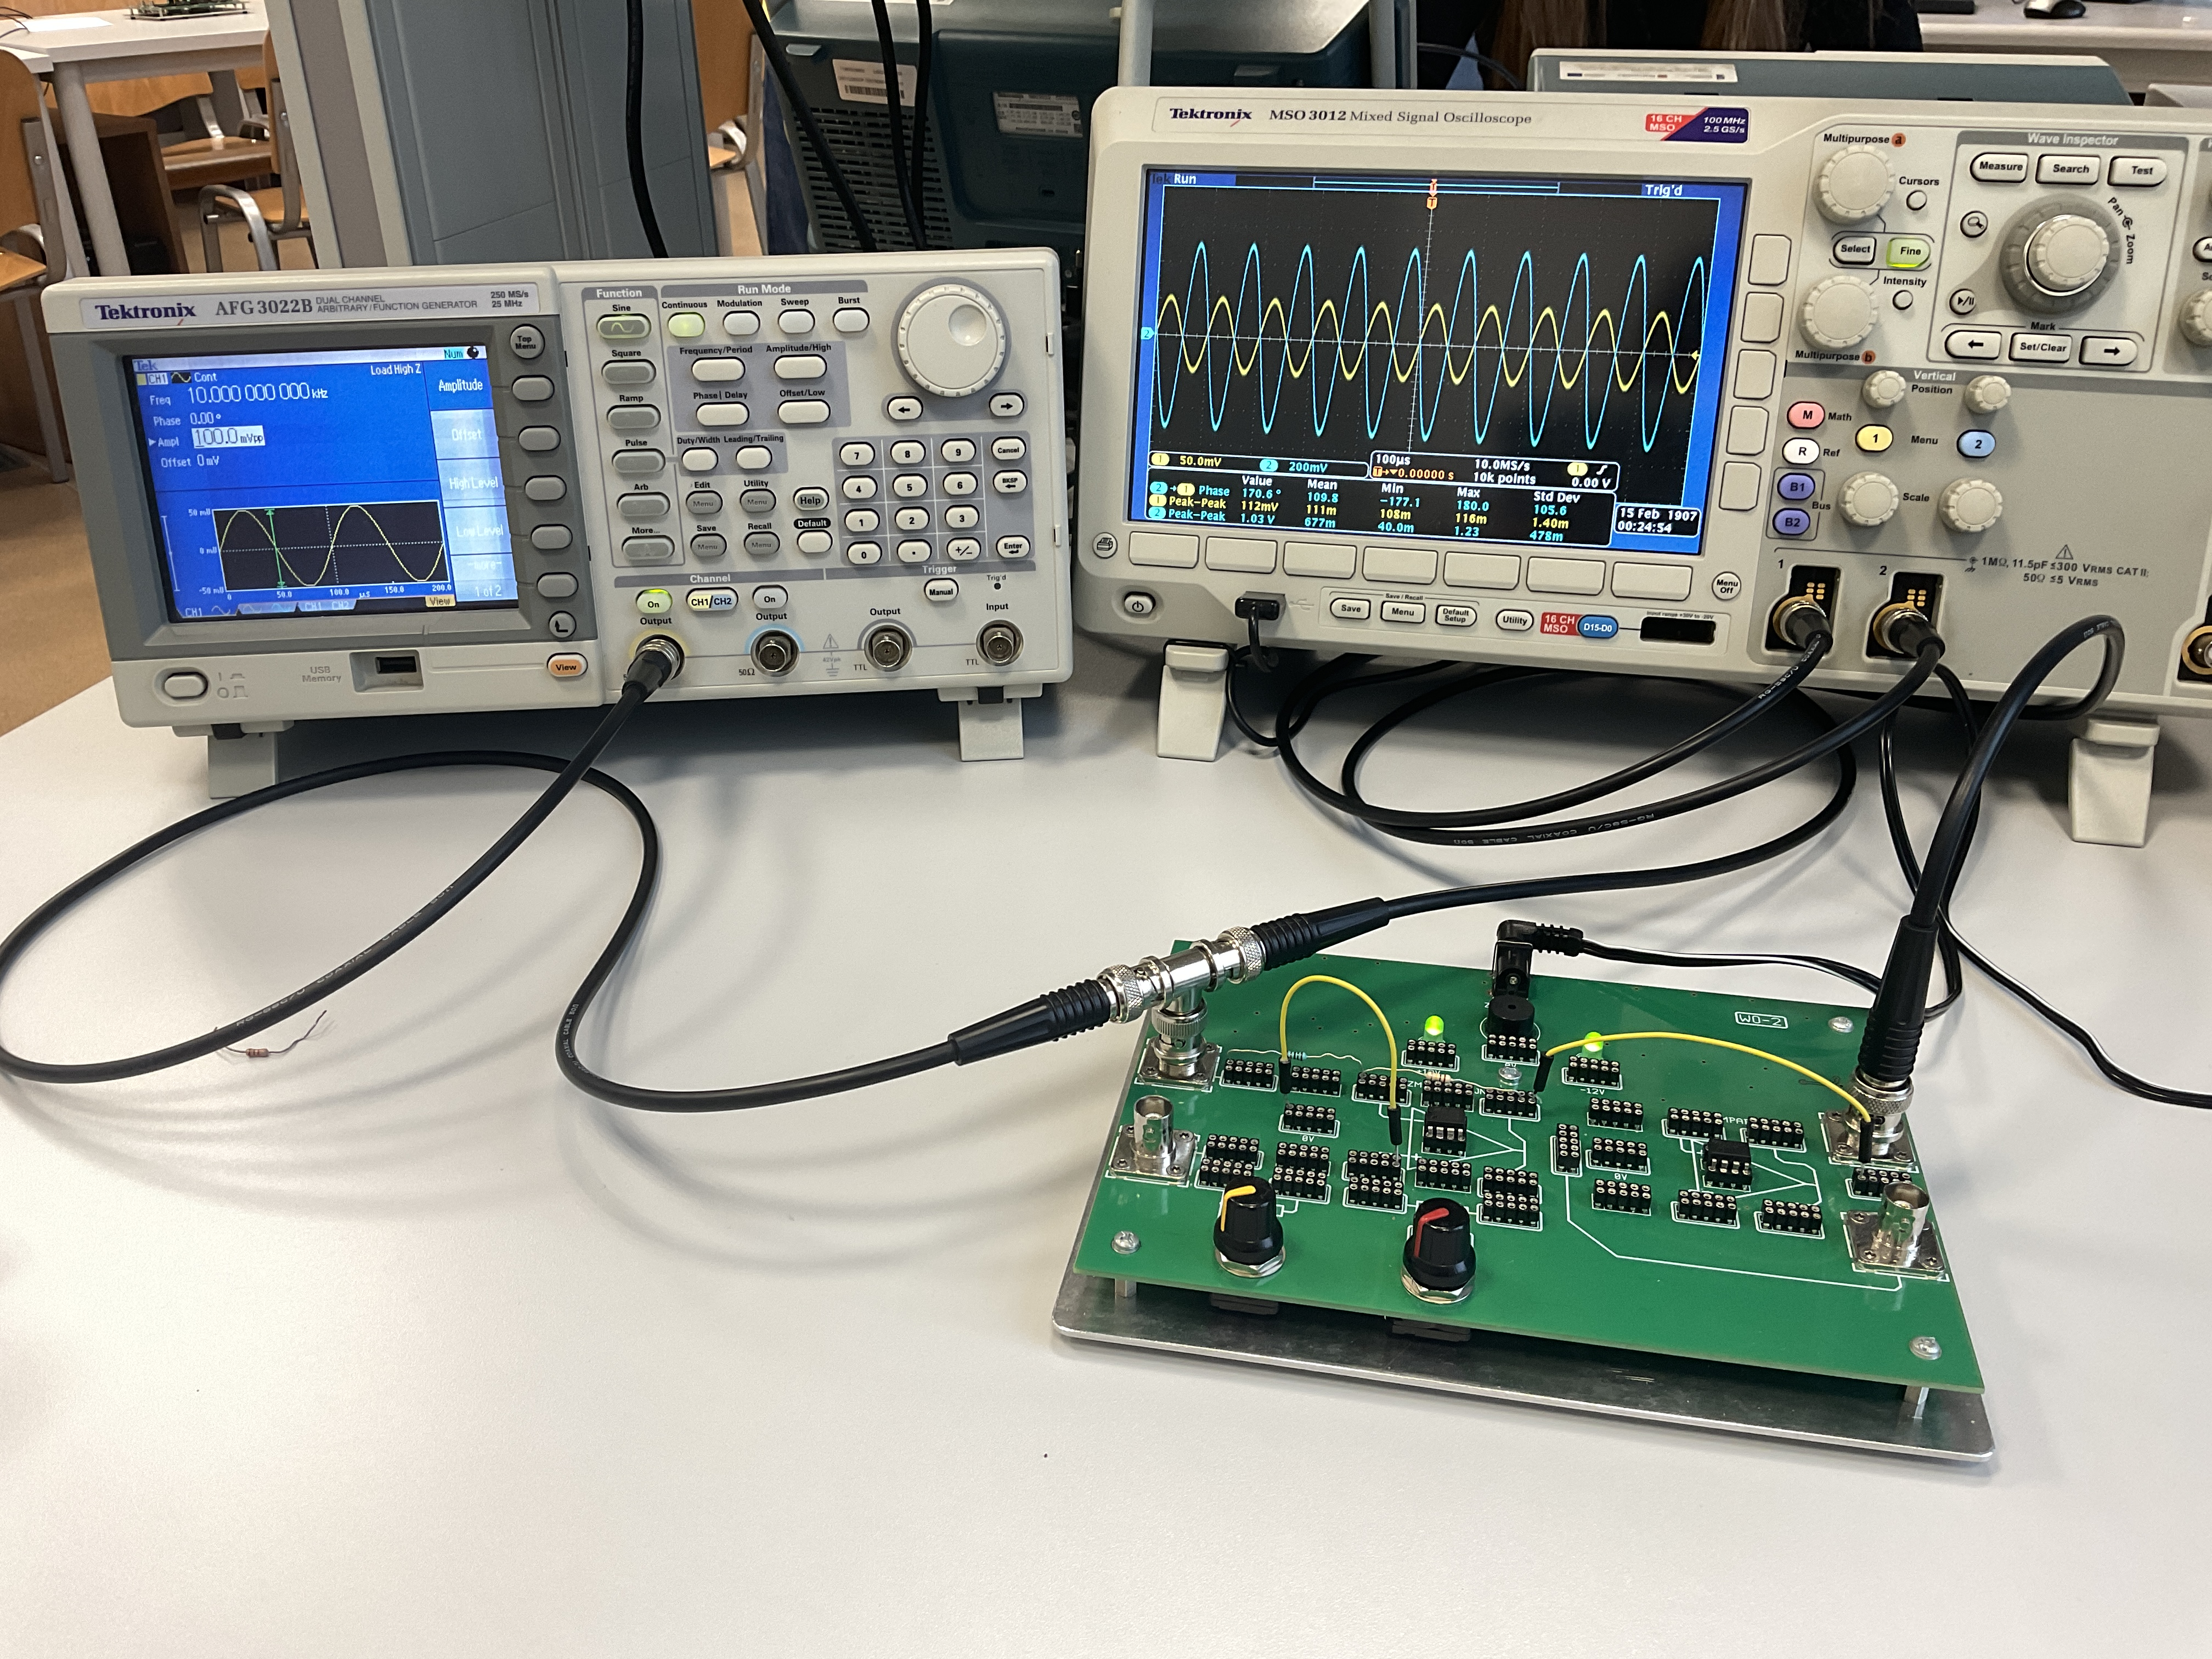
\includegraphics[width=7cm]{C2}
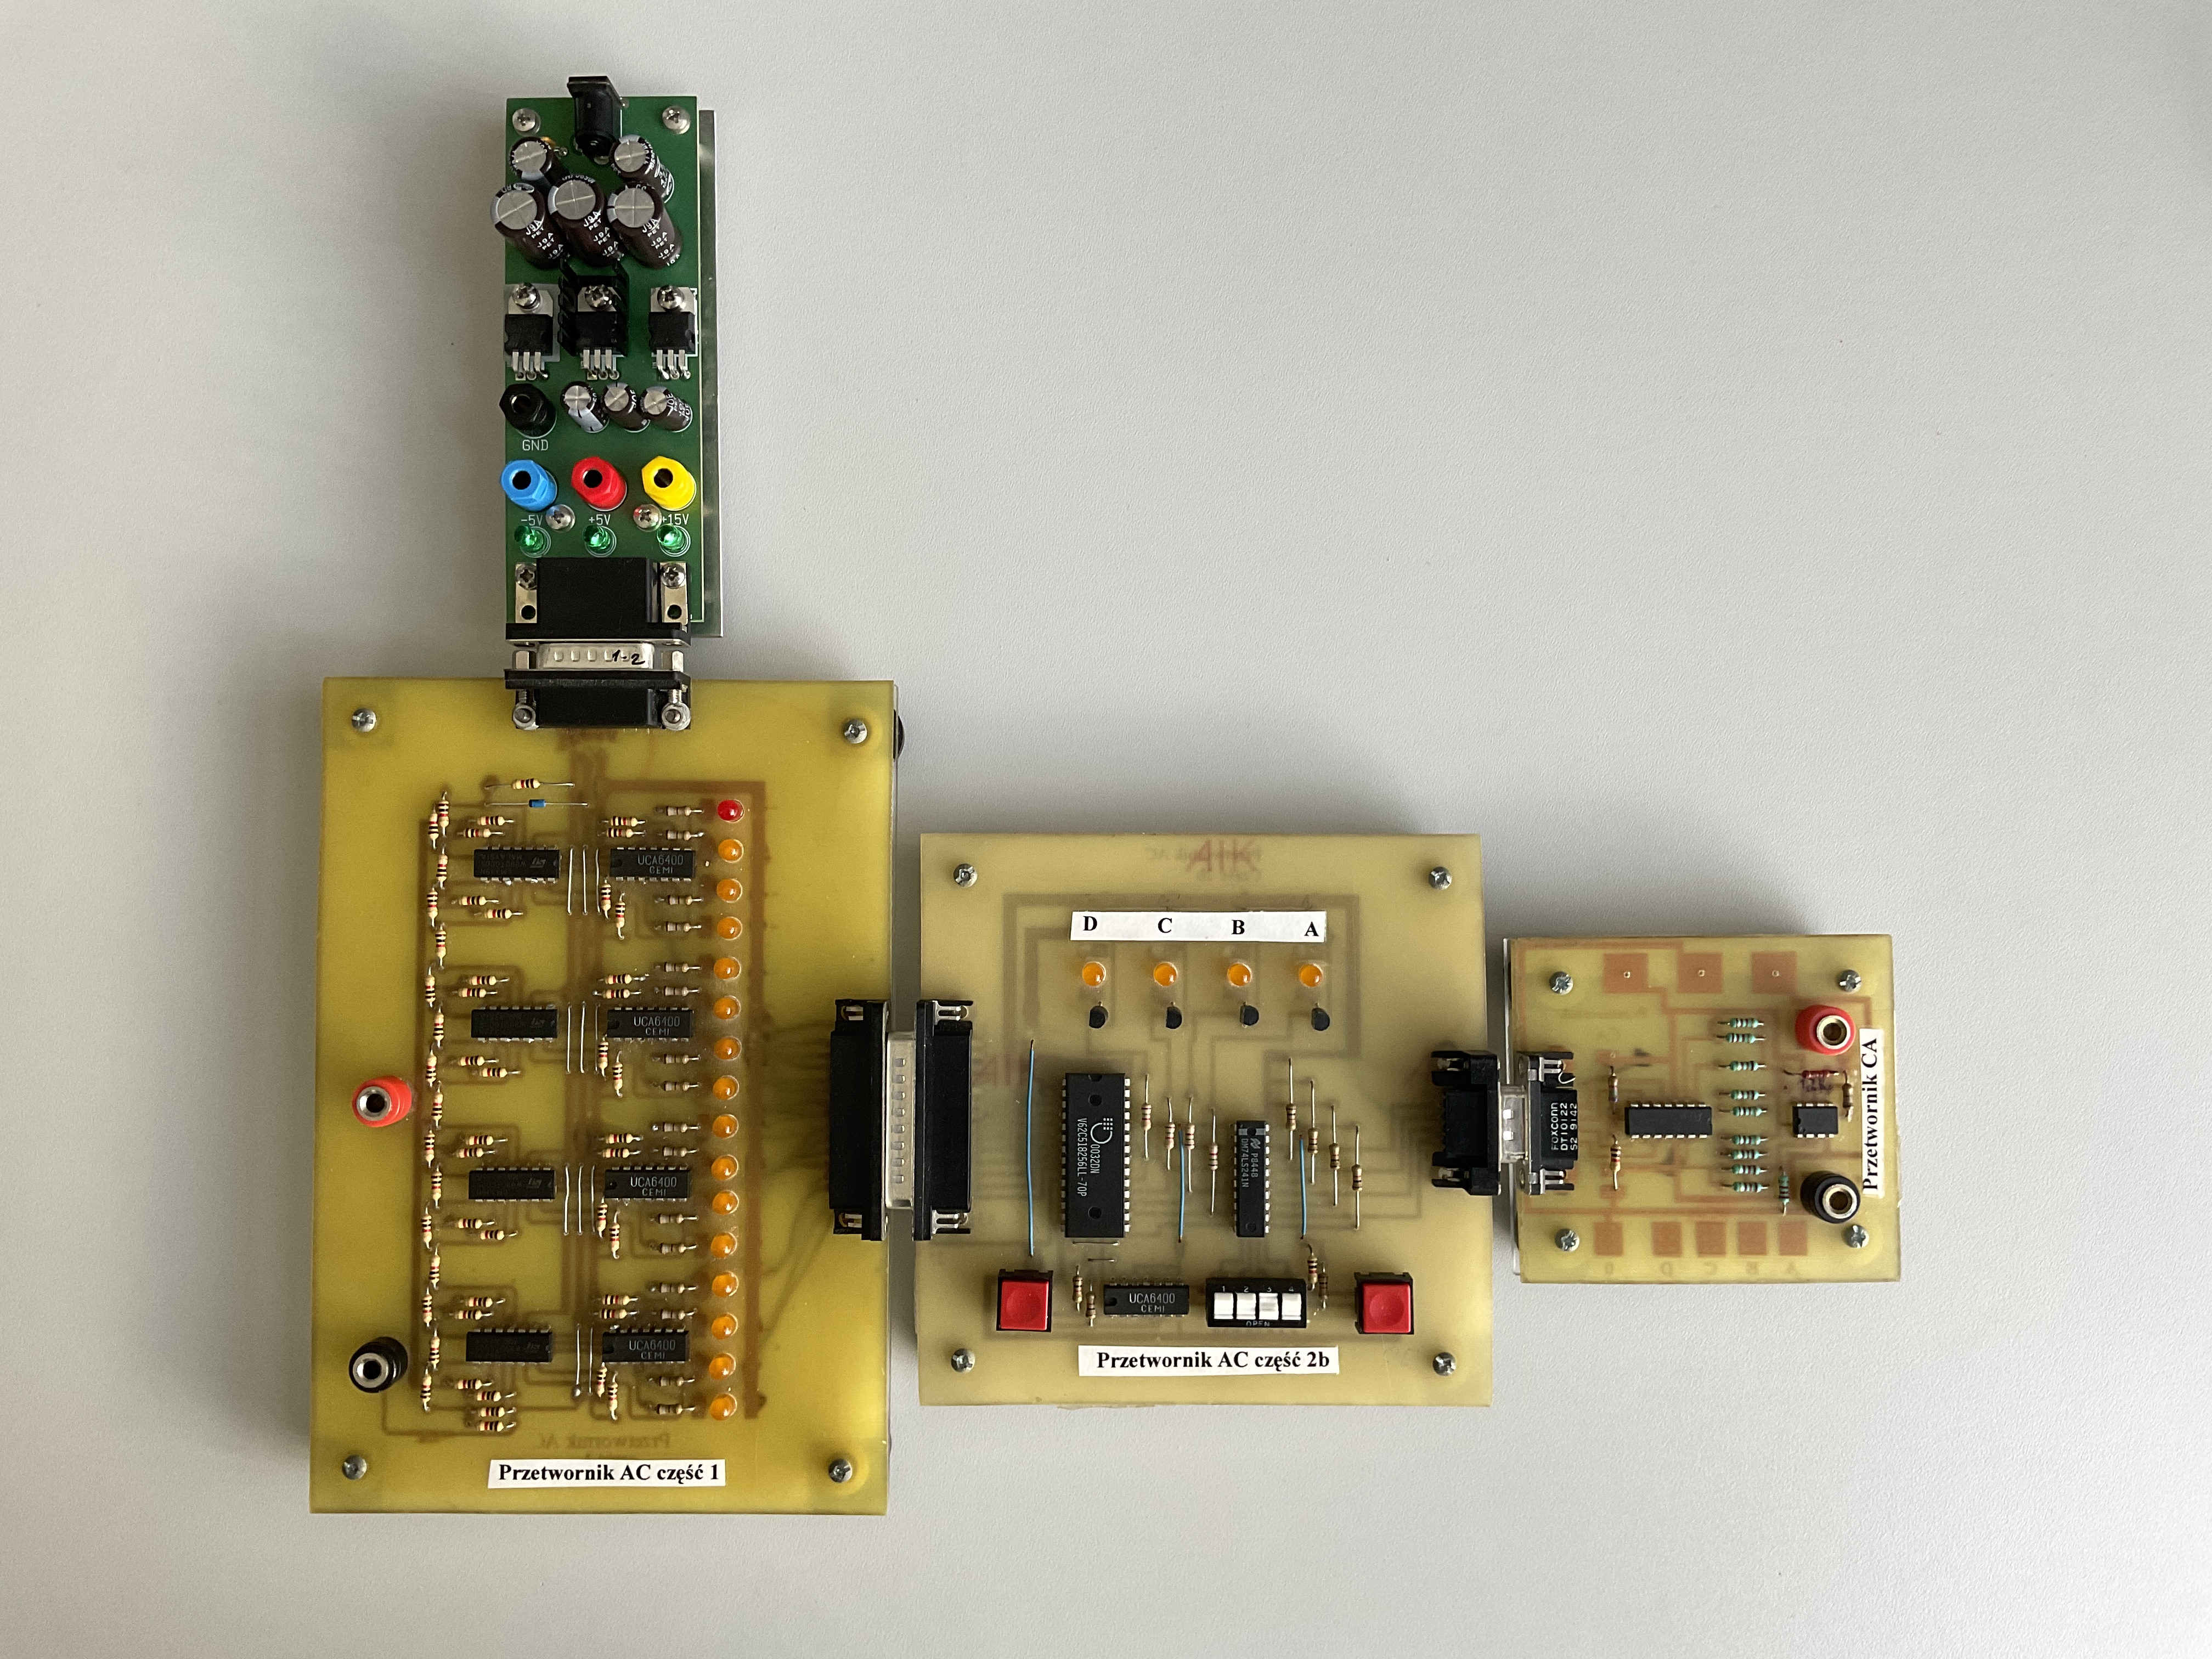
\includegraphics[width=7cm]{C3}
\centering
\captionsetup{labelformat=empty}
\caption{}
\end{figure}

Zbadane pzeze mnie przebiegi wyjścia $Q$ w zależności od wejść CLK, CLR, PRE i D wyglądały następująco:

\begin{center}
\begin{tikzpicture}

	\node (CLK) at (-1, 9) {CLK}; 
	\node (D) at (-1, 7) {D};
	\node (CLR) at (-1, 5) {CLR};
	\node (PRE) at (-1, 3) {PRE};
	\node (Q) at (-1, 1) {Q};

	\draw [cyan, thick] (0, 8.5)--(3, 8.5)--(3, 9.5)--(6, 9.5)--(6, 8.5)--(9, 8.5)--(9, 9.5)--(12, 9.5)--(12, 8.5)--(15, 8.5)--(15, 9.5)--(15.2, 9.5);

	\draw [magenta, thick] (0, 6.5)--(2, 6.5)--(2, 7.5)--(4, 7.5)--(4, 6.5)--(7, 6.5)--(7, 7.5)--(7.3, 7.5)--(7.3, 6.5)--(8, 6.5)--(8, 7.5)--(9.5, 7.5)--(9.5, 6.5)--(10, 6.5)--(10, 7.5)--(10.2, 7.5)--(10.2, 6.5)--(15.2, 6.5);

	\draw [red, thick] (0, 5.5)--(15.2, 5.5);
	\draw [thick](0, 3.5)--(15.2, 3.5);

	\draw [blue, thick] (0, 0.5)--(3, 0.5)--(3, 1.5)--(6, 1.5)--(6, 0.5)--(9, 0.5)--(9, 1.5)--(9.5, 1.5)--(9.5, 0.5)--(10, 0.5)--(10, 1.5)--(10.2, 1.5)--(10.2, 0.5)--(15.2, 0.5);

\end{tikzpicture}
\end{center}

\newpage
\begin{center}
\begin{tikzpicture}

	\node (CLK) at (-1, 9) {CLK}; 
	\node (D) at (-1, 7) {D};
	\node (CLR) at (-1, 5) {CLR};
	\node (PRE) at (-1, 3) {PRE};
	\node (Q) at (-1, 1) {Q};

	\draw [cyan, thick] (0, 8.5)--(3, 8.5)--(3, 9.5)--(6, 9.5)--(6, 8.5)--(9, 8.5)--(9, 9.5)--(12, 9.5)--(12, 8.5)--(15, 8.5)--(15, 9.5)--(15.2, 9.5);

	\draw [magenta, thick] (0, 6.5)--(2, 6.5)--(2, 7.5)--(4, 7.5)--(4, 6.5)--(7, 6.5)--(7, 7.5)--(7.3, 7.5)--(7.3, 6.5)--(8, 6.5)--(8, 7.5)--(9.5, 7.5)--(9.5, 6.5)--(10, 6.5)--(10, 7.5)--(10.2, 7.5)--(10.2, 6.5)--(15.2, 6.5);

	\draw [red, thick] (0, 5.5)--(5.2, 5.5)--(5.2, 4.5)--(5.4, 4.5)--(5.4, 5.5)--(15.2, 5.5);
	\draw [thick] (0, 3.5)--(15.2, 3.5);

	\draw [blue, thick] (0, 0.5)--(3, 0.5)--(3, 1.5)--(5.2, 1.5)--(5.2, 0.5)--(9, 0.5)--(9, 1.5)--(9.5, 1.5)--(9.5, 0.5)--(10, 0.5)--(10, 1.5)--(10.2, 1.5)--(10.2, 0.5)--(15.2, 0.5);

\end{tikzpicture}
\end{center}

\vspace{4cm}

\begin{center}
\begin{tikzpicture}

	\node (CLK) at (-1, 9) {CLK}; 
	\node (D) at (-1, 7) {D};
	\node (CLR) at (-1, 5) {CLR};
	\node (PRE) at (-1, 3) {PRE};
	\node (Q) at (-1, 1) {Q};

	\draw [cyan, thick] (0, 8.5)--(3, 8.5)--(3, 9.5)--(6, 9.5)--(6, 8.5)--(9, 8.5)--(9, 9.5)--(12, 9.5)--(12, 8.5)--(15, 8.5)--(15, 9.5)--(15.2, 9.5);

	\draw [magenta, thick] (0, 6.5)--(2, 6.5)--(2, 7.5)--(4, 7.5)--(4, 6.5)--(7, 6.5)--(7, 7.5)--(7.3, 7.5)--(7.3, 6.5)--(8, 6.5)--(8, 7.5)--(9.5, 7.5)--(9.5, 6.5)--(10, 6.5)--(10, 7.5)--(10.2, 7.5)--(10.2, 6.5)--(15.2, 6.5);

	\draw [red, thick] (0, 5.5)--(15.2, 5.5);
	\draw [thick](0, 3.5)--(13, 3.5)--(13, 2.5)--(13.2, 2.5)--(13.2, 3.5)--(15.2, 3.5);

	\draw [blue, thick] (0, 0.5)--(3, 0.5)--(3, 1.5)--(6, 1.5)--(6, 0.5)--(9, 0.5)--(9, 1.5)--(9.5, 1.5)--(9.5, 0.5)--(10, 0.5)--(10, 1.5)--(10.2, 1.5)--(10.2, 0.5)--(13, 0.5)--(13, 1.5)--(15.2, 1.5);

\end{tikzpicture}
\end{center}

\newpage
Na podstawie tych obserwacji można więc wnioskować, że tabela stanów logicznych układu 7474 wygląda następująco:

\begin{center}
\begin{tabular}{ | c | c | c | c | c |}
\hline
PRE & CLR & CLK & \ \ D \ \ & \ \ $Q$ \ \ \\
\hline
\hline
0 & 0 & \textit{x} & \textit{x} & - \\
\hline
0 & 1 & \textit{x} & \textit{x} & 1 \\
\hline
1 & 0 & \textit{x} & \textit{x} & 0 \\
\hline
1 & 1 & 0 &  \textit{x} & \textit{p} \\
\hline
1 & 1 & 1 & 0 & 0 \\
\hline
1 & 1 & 1 & 1 & 1 \\
\hline
\end{tabular}
\end{center}

gdzie \textit{p} oznacza stan pamiętania, - oznacza stan niedozwolony, a \textit{x} oznacza dowolną wartość logiczną (czyli, że w danej chwili wartość wyjścia $Q$ nie zależy od stanu tego wejścia).

\newpage
\paragraph{Ćwiczenie 5.3 \\}

Zbadanie działania przerzutnika \textit{D-latch} (układ scalony 7475), podając na odpowiednie wejścia sygnał zegara lub sygnały z impulsatora. \\

Układ przerzutnika D-latch znajdującego się na układach 7475 można przedstawić schematycznie tak:

\begin{center}
\begin{circuitikz} [circuit logic US, scale=2]
	
	\ctikzset{multipoles/dipchip/pin spacing=0.5}
	\node [anchor=pin 1, dipchip, num pins=6, hide numbers, no topmark, external pins width=0, scale=2](d1){};

	\node [right] at (d1.bpin 1) {\textsl{CLK}};
	\node [right] at (d1.bpin 3) {\textsl{D}};
	\node [left] at (d1.bpin 6) {\textsl{Q}};
	\node [left] at (d1.bpin 4) {\textsl{\ctikztextnot{Q}}};

	\draw (d1.bpin 1) -- ++(left: 0.7);
	\draw (d1.bpin 3) -- ++(left: 0.7);
	\draw (d1.bpin 4) -- ++(right: 0.7);
	\draw (d1.bpin 6) -- ++(right: 0.7);

\end{circuitikz}
\end{center}

Skonstruowałem następujący układ: wyjście $Q$ przerzutnika podłączyłem pod próbnik stanów logicznych. Wyjście pierwszego impulsatora podpiąłem pod wejście zegarowe CLK oraz diodę sygnalizującą stan zegara. Wejście drugiego impulsatora podłączyłem do wejścia D przerzutnika.

\begin{figure}[H]
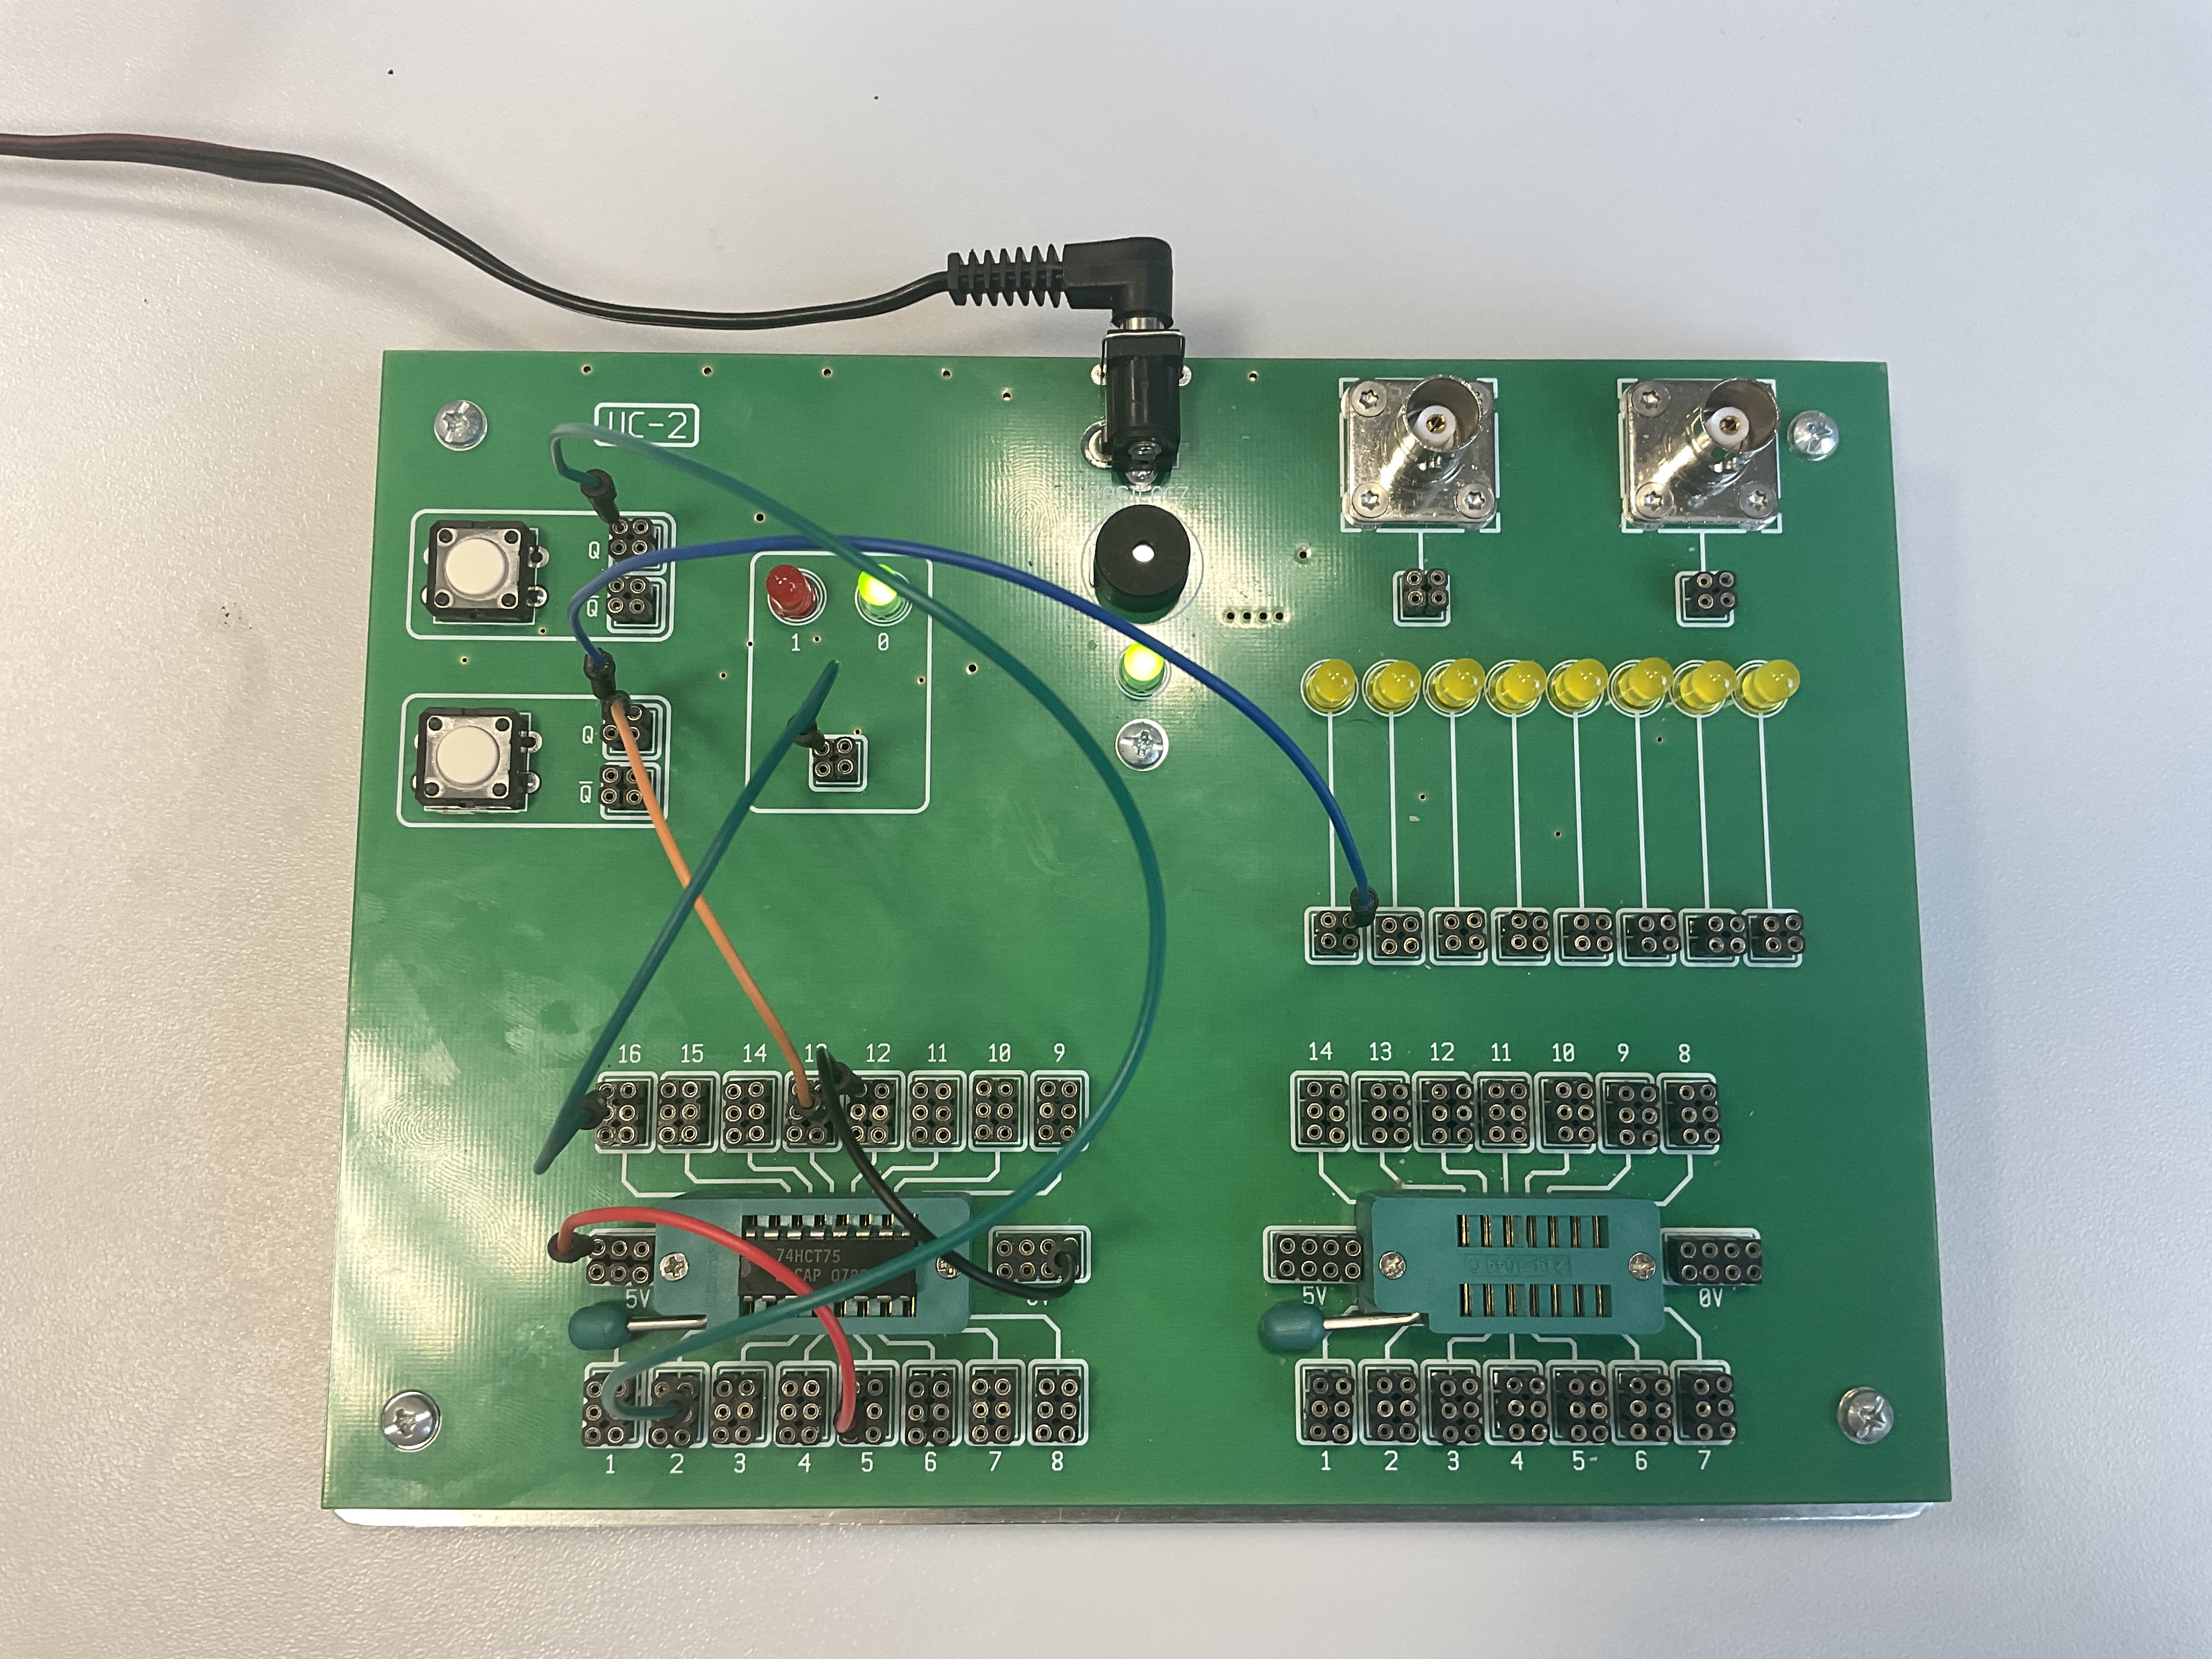
\includegraphics[width=15cm]{C4}
\centering
\captionsetup{labelformat=empty}
\caption{}
\end{figure}

\newpage
Zmieniając stany obydwu wejść obserwowałem wartości na wyjściu $Q$. Zdjęcia załączam w pliku \texttt{Sprawozdanie-cwiczenie5-Jan-Kwinta-Zalacznik2.zip}. Przebiegi, które obserwowałem na wyjściu w zależności od wejść CLK i D wyglądały następująco:

\begin{center}
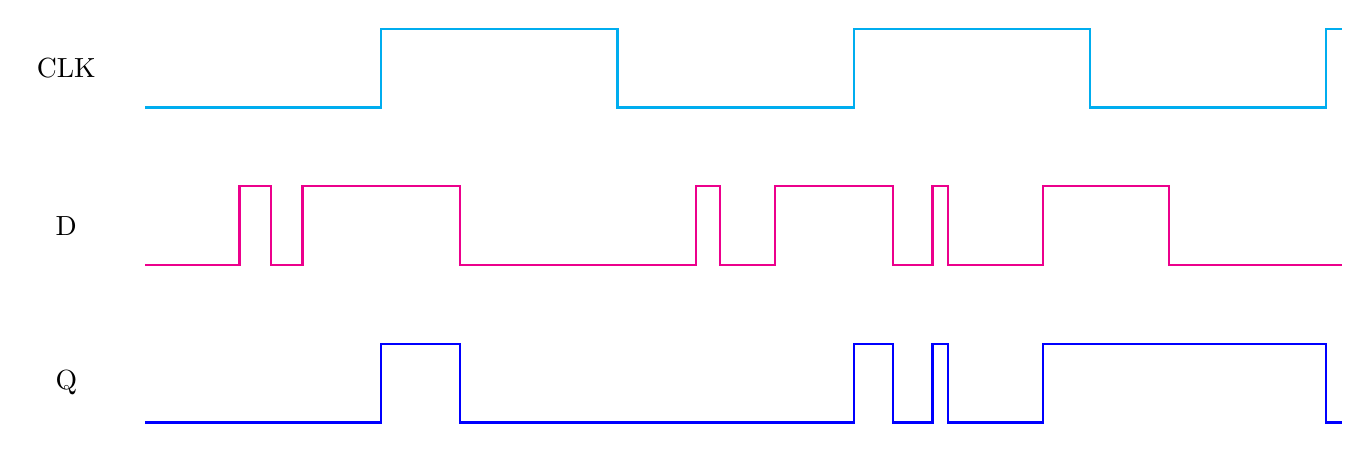
\begin{tikzpicture}

	\node (CLK) at (-1, 9) {CLK}; 
	\node (D) at (-1, 7) {D};
	\node (Q) at (-1, 5) {Q};

	\draw [cyan, thick] (0, 8.5)--(3, 8.5)--(3, 9.5)--(6, 9.5)--(6, 8.5)--(9, 8.5)--(9, 9.5)--(12, 9.5)--(12, 8.5)--(15, 8.5)--(15, 9.5)--(15.2, 9.5);

	\draw [magenta, thick] (0, 6.5)--(1.2, 6.5)--(1.2, 7.5)--(1.6, 7.5)--(1.6, 6.5)--(2, 6.5)--(2, 7.5)--(4, 7.5)--(4, 6.5)--(7, 6.5)--(7, 7.5)--(7.3, 7.5)--(7.3, 6.5)--(8, 6.5)--(8, 7.5)--(9.5, 7.5)--(9.5, 6.5)--(10, 6.5)--(10, 7.5)--(10.2, 7.5)--(10.2, 6.5)--(11.4, 6.5)--(11.4, 7.5)--(13, 7.5)--(13, 6.5)--(15.2, 6.5);

	\draw [blue, thick] (0, 4.5)--(3, 4.5)--(3, 5.5)--(4, 5.5)--(4, 4.5)--(9, 4.5)--(9, 5.5)--(9.5, 5.5)--(9.5, 4.5)--(10, 4.5)--(10, 5.5)--(10.2, 5.5)--(10.2, 4.5)--(11.4, 4.5)--(11.4, 5.5)--(15, 5.5)--(15, 4.5)--(15.2, 4.5);

\end{tikzpicture}
\end{center}

Na podstawie tych pomiarów można wywnioskować tabelę stanów logicznych układu 7475:

\begin{center}
\begin{tabular}{| c | c | c |}
\hline
CLK & \ \ D \ \ & \ \ $Q$ \ \ \\
\hline
\hline
0 & \textit{x} & \textit{p} \\
\hline
1 & 0 & 0 \\
\hline
1 & 1 & 1 \\
\hline
\end{tabular}
\end{center}

gdzie \textit{p} oznacza stan pamiętania, a \textit{x} oznacza dowolną wartość. \\

Największa różnica pomiędzy przerzutnikiem \textit{D-latch} wyzwalanym po- ziomem a przerzutnikiem synchronicznym RS jest taka, że \textit{D-latch} nie posiada stanów zabronionych. Analizując tabelę stanów logicznych obydwu tych przerzutników można dojść do wniosku, że gdyby spiąć razem wejścia przerzutnika RS zaprzeczając jedno z nich (np. $S$ i $\overline{R}$) to otrzymalibyśmy właśnie przerzutnik D wyzwalany poziomem.

\newpage
\paragraph{Ćwiczenie 5.4 \\}

Zmontowanie, w oparciu o przerzutnik JK (7493) układu dzielącego częstotliwość przez dwa. \\

Przerzutnik JK można schematycznie przedstawić schematycznie:

\begin{center}
\begin{circuitikz} [circuit logic US, scale=2]
	
	\ctikzset{multipoles/dipchip/pin spacing=0.5}
	\node [anchor=pin 1, dipchip, num pins=8, hide numbers, no topmark, external pins width=0, scale=2](d1){};

	\node [right] at (d1.bpin 1) {\textsl{J}};
	\node [right] at (d1.bpin 2) {\textsl{CLK}};
	\node [right] at (d1.bpin 3) {\textsl{RST}};
	\node [right] at (d1.bpin 4) {\textsl{K}};
	\node [left] at (d1.bpin 8) {\textsl{Q}};
	\node [left] at (d1.bpin 5) {\textsl{\ctikztextnot{Q}}};

	\draw (d1.bpin 1) -- ++(left: 0.7);
	\draw (d1.bpin 2) -- ++(left: 0.7);
	\draw (d1.bpin 3) -- ++(left: 0.7);
	\draw (d1.bpin 4) -- ++(left: 0.7);
	\draw (d1.bpin 5) -- ++(right: 0.7);
	\draw (d1.bpin 8) -- ++(right: 0.7);

\end{circuitikz}
\end{center}

Przerzutnik ma wejścia informacyjne J i K, zegarowe CLK, wyjście $Q$ i jego negację $\overline{Q}$. Posiada także asynchroniczne wejście resetujące RST. \\

Podanie jedynki logicznej na wejście J powoduje ustawienie przerzutnika (co skutkuje pojawieniem się stanu wysokiego na wyjściu Q). Ustawienie wejścia K w stan wysoki przestawia przerzutnik w stan niski. Jeżeli jedynka logiczna zostanie ustawiona na obydwu wejściach J i K to nastąpi zmiana stanu przerzutnika na przeciwny (czyli jeżeli układ był w stanie wysokim to przejdzie w stan niski i odwrotnie). JK jest przerzutnikiem synchronicznym, co oznacza, że reaguje na stan wejść tylko przy podaniu odpowiedniego sygnału na wejście zegarowe. \\

Na układach scalonych 7493 wejścia J oraz K "na sztywno" spiętę są z $5 \ V$, czyli logiczną jedynką. Sprawia to, że za każdym razem, kiedy na wejściu zegarowym zmienia się sygnał z 0 na 1 to przerzutnik zmienia stan wyjścia $Q$. Zamienia to nasz przerzutnik JK w dokładnie taki układ, jaki jest nam potrzebny do zadania — jeżeli $Q$ przerzutnika JK będzie zmieniało stan za każdym razem, kiedy na zegarze będzie zbocze rosnące, znaczy, że $Q$ będzie miało dwa razy mniejszą częstotliwość niż wejście CLK.

\newpage

\begin{figure}[H]
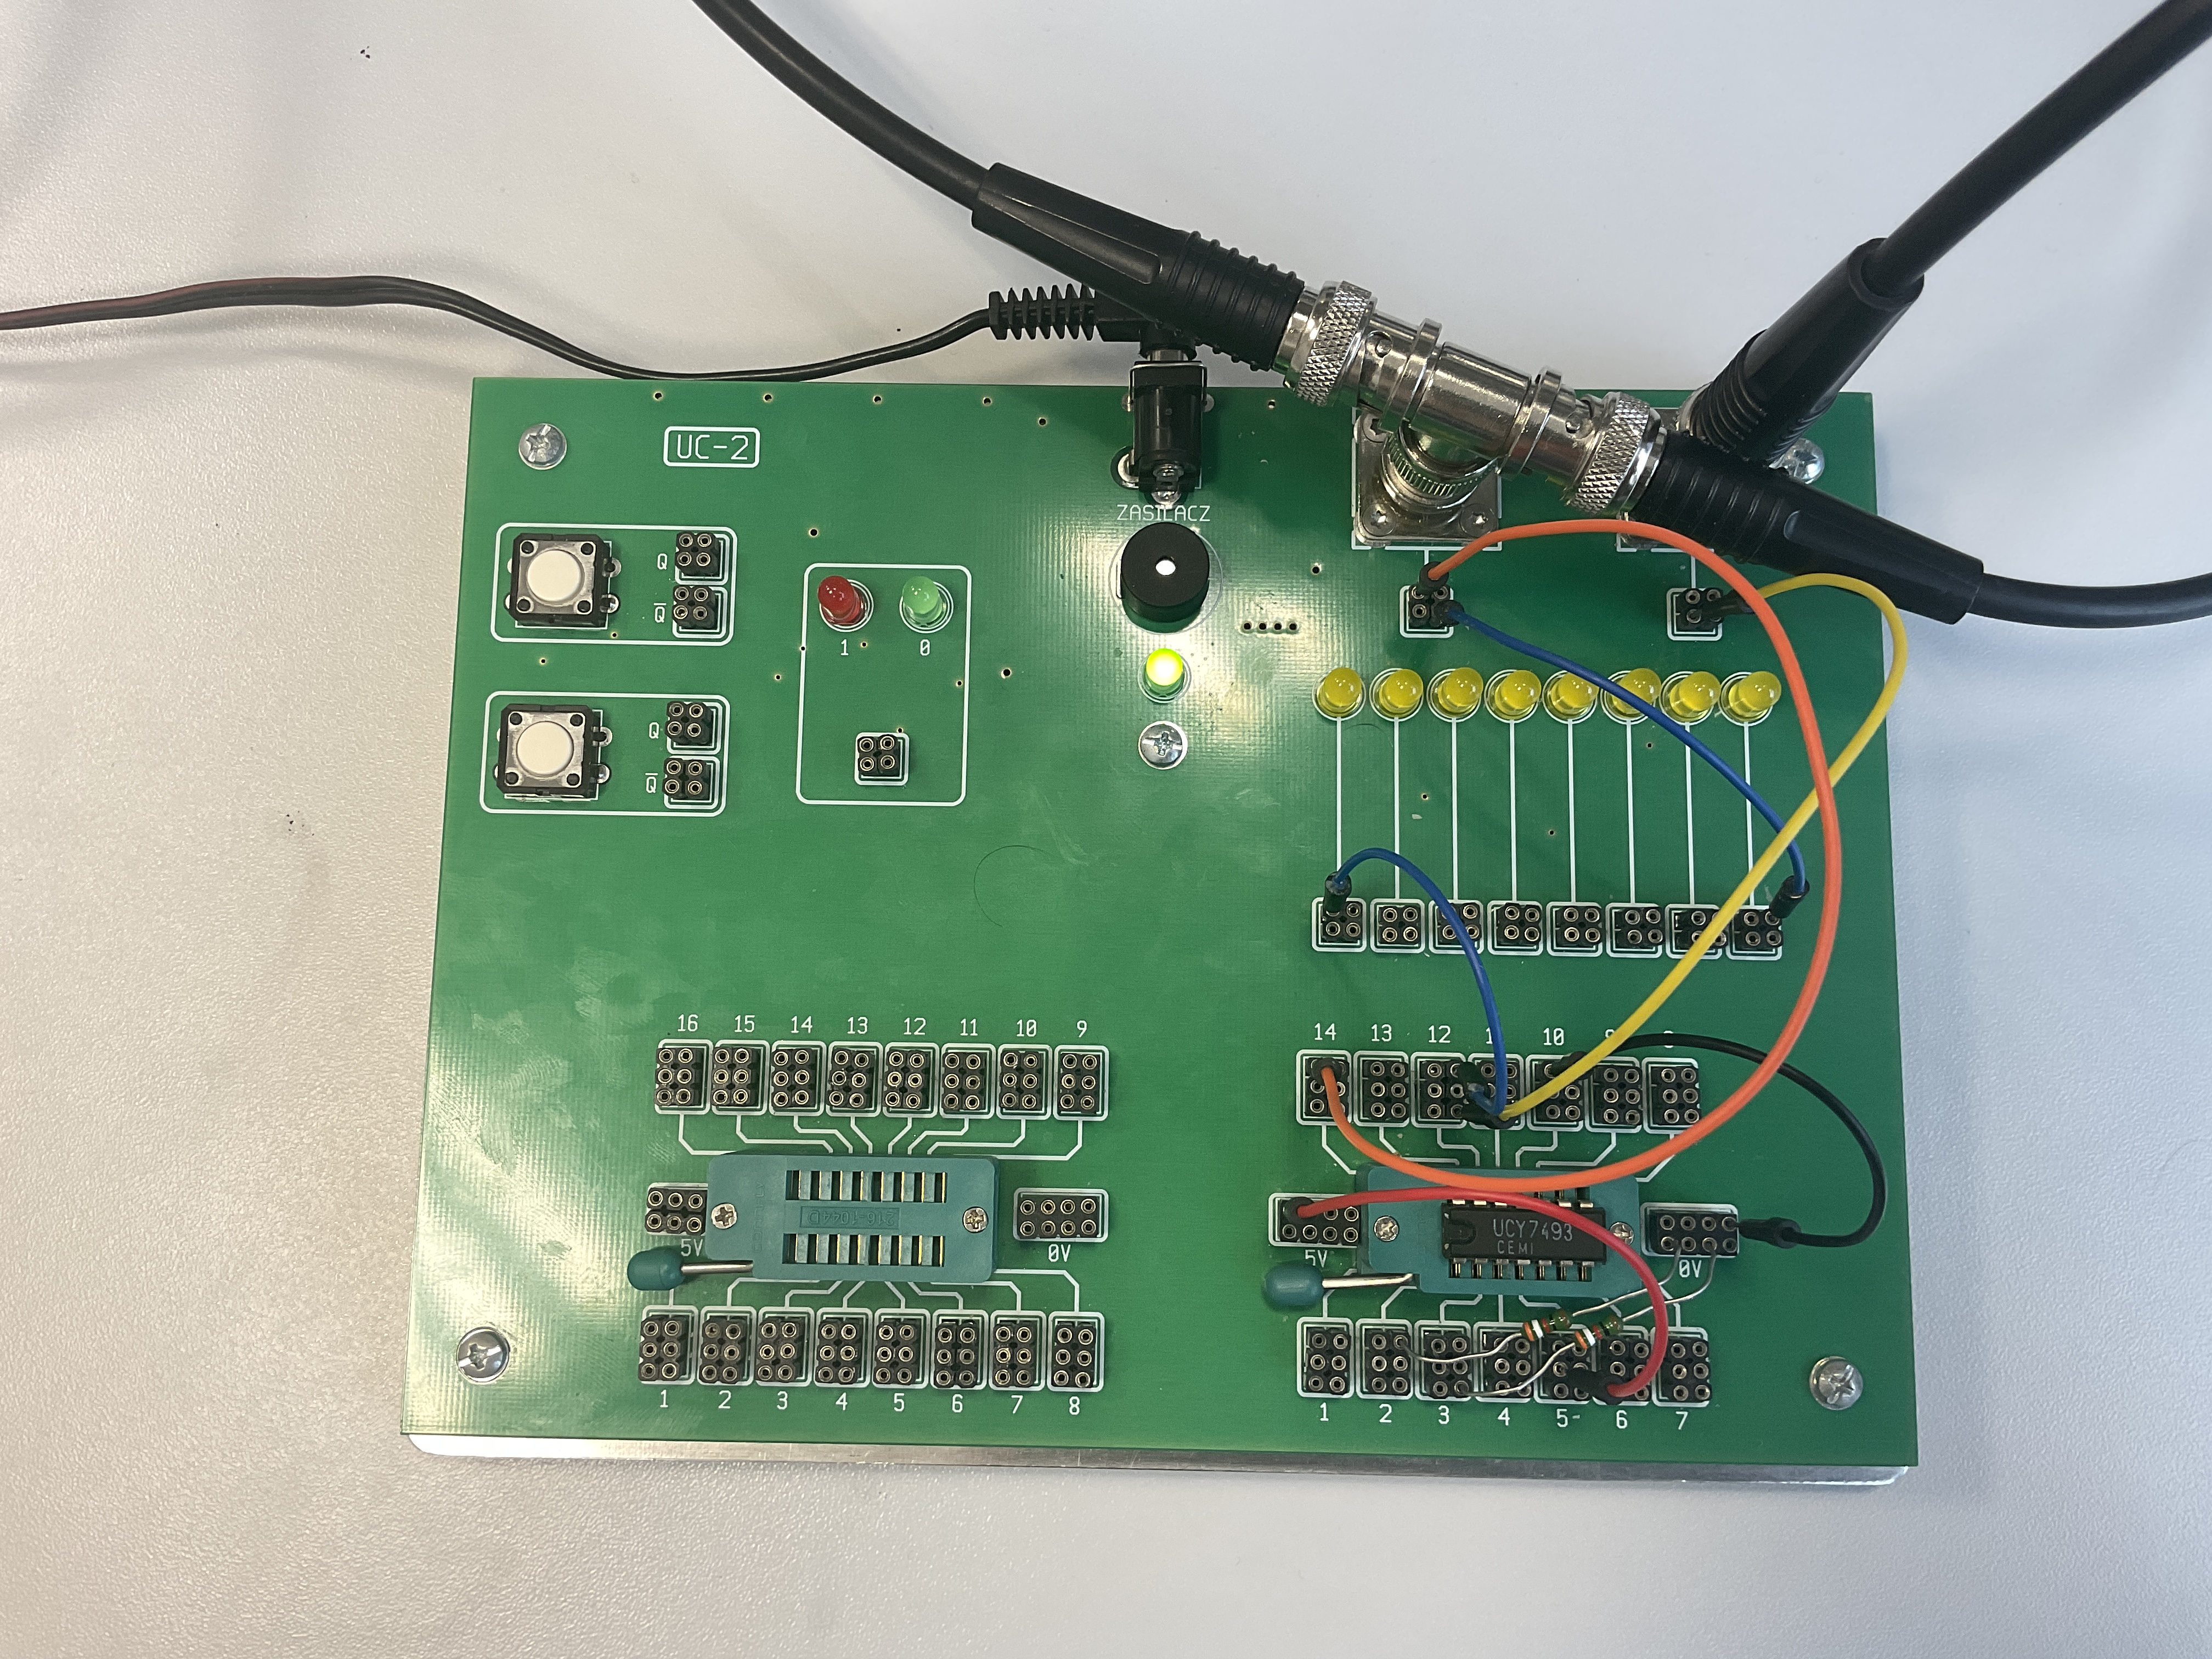
\includegraphics[width=8cm]{C5}
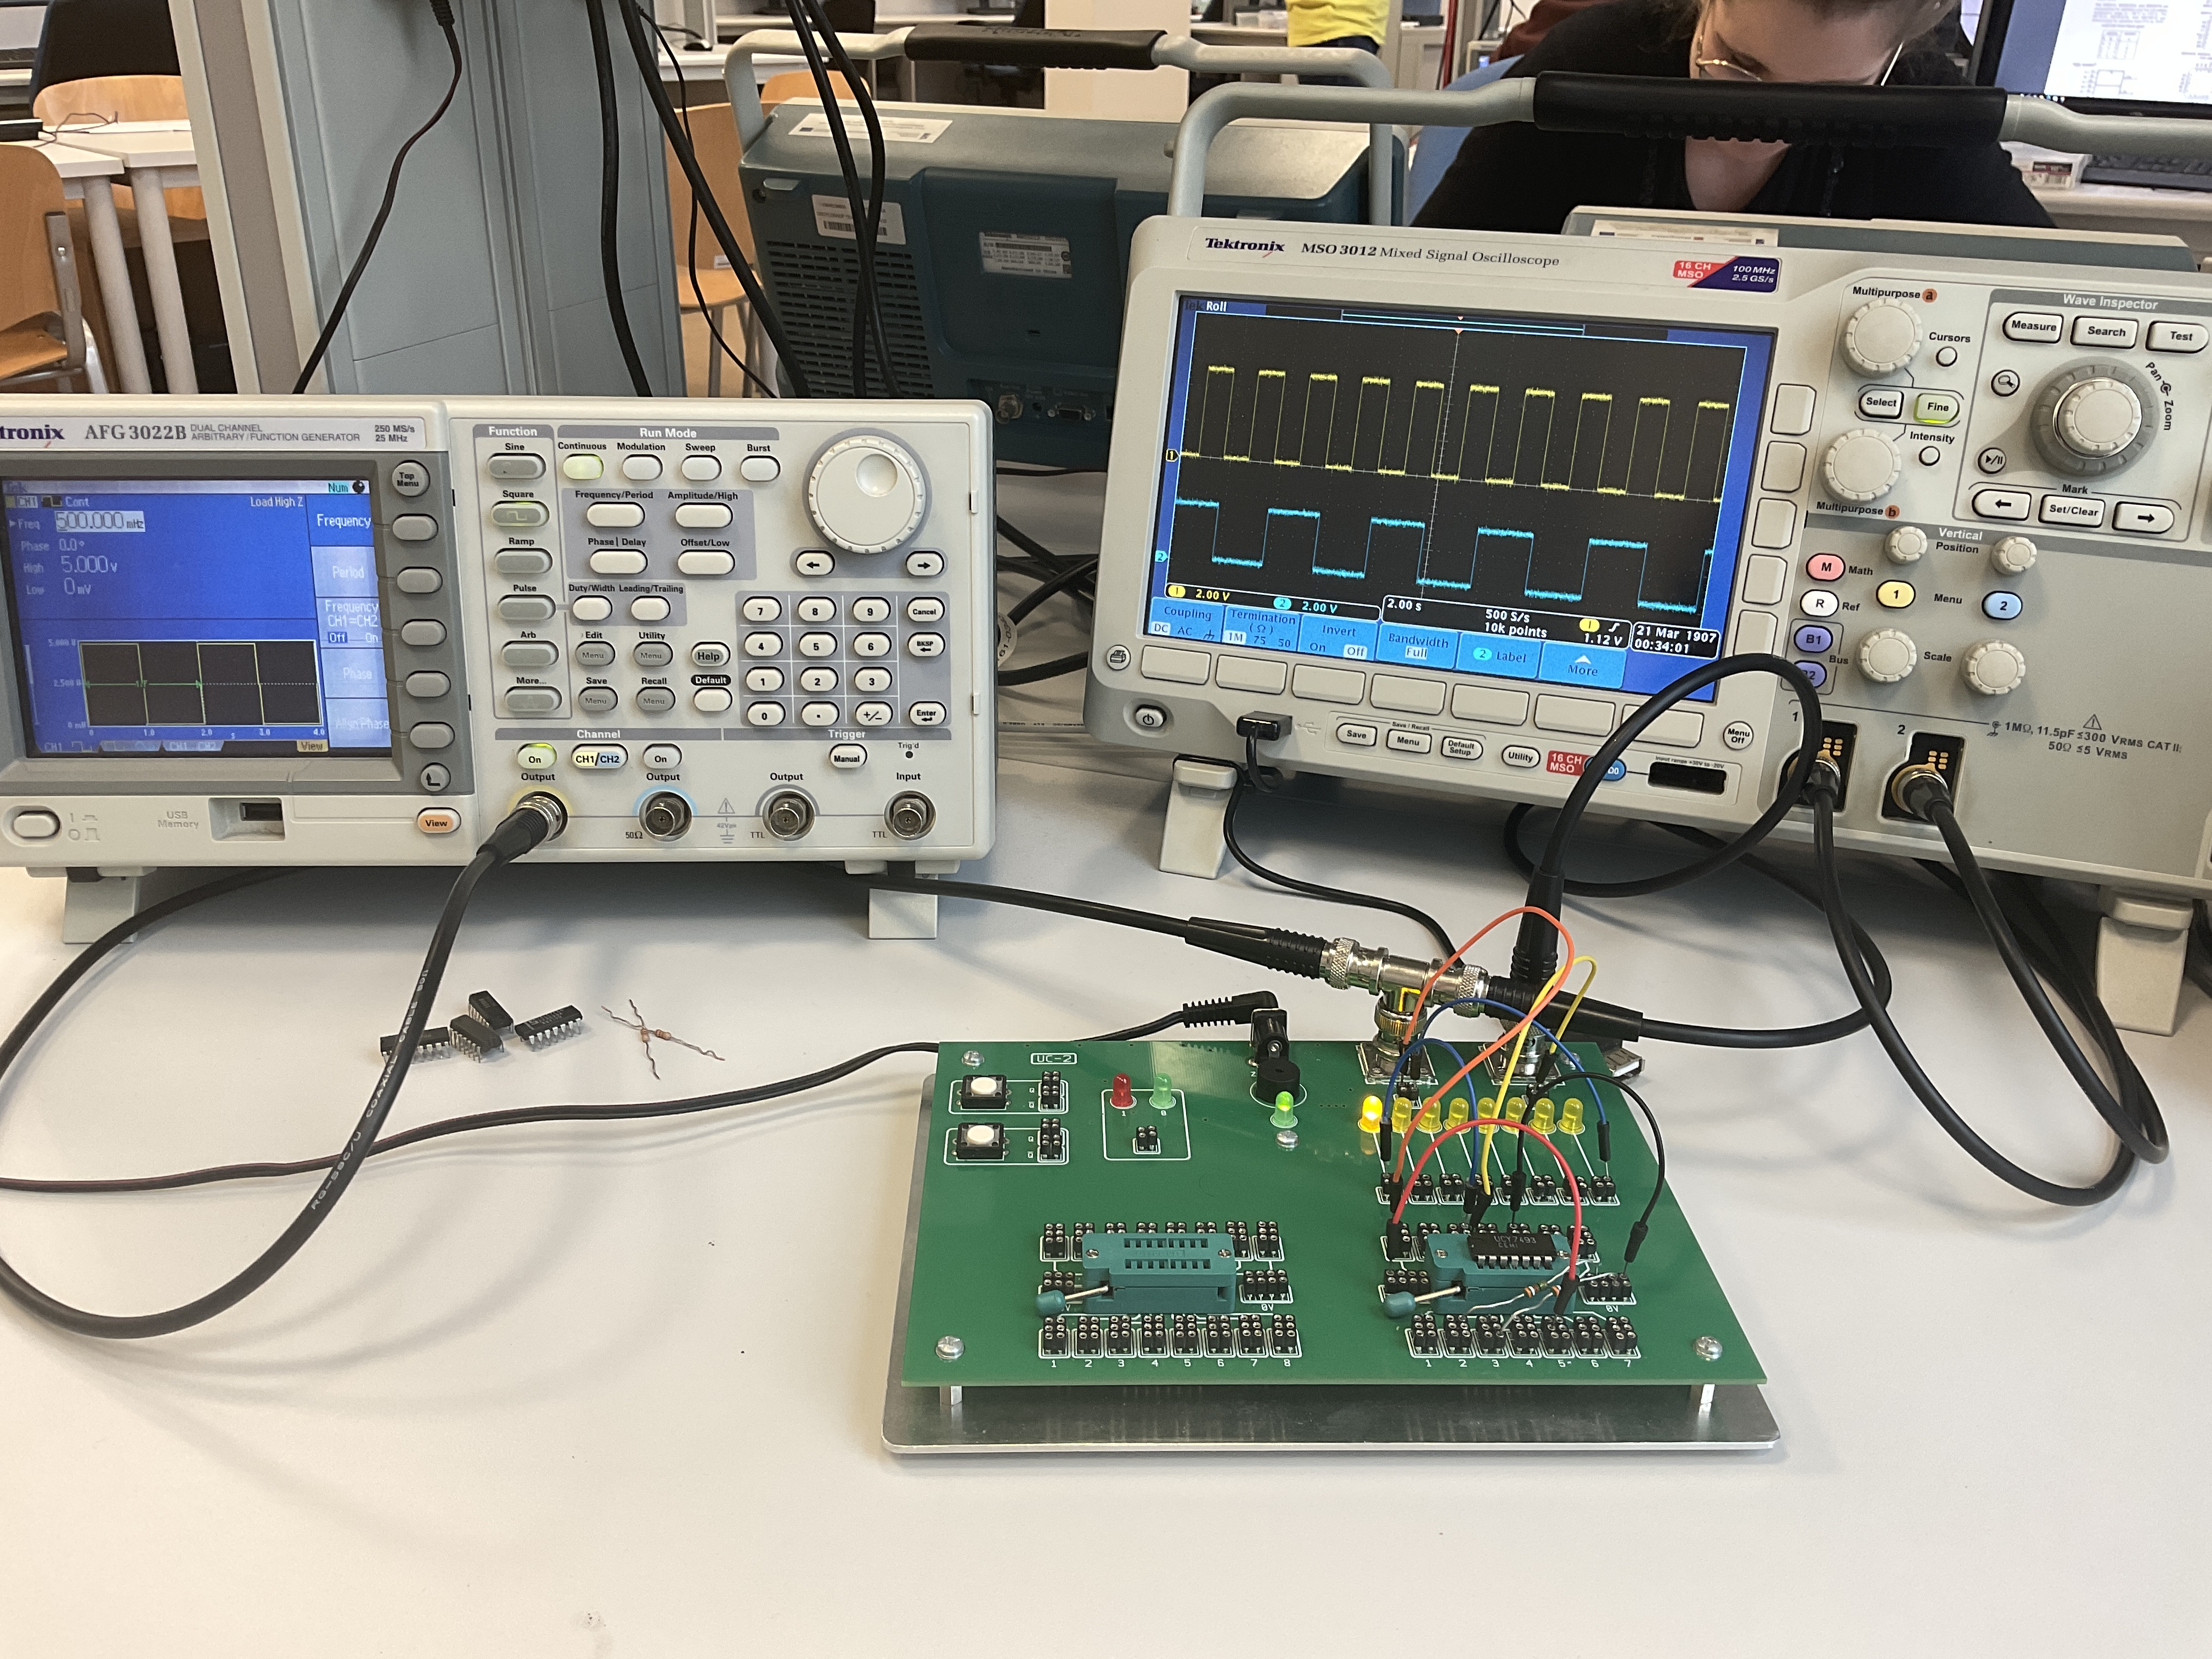
\includegraphics[width=8cm]{C6}
\centering
\captionsetup{labelformat=empty}
\caption{}
\end{figure}

Zmontowałem powyższy układ i podałem na wejście zegarowe sygnał z generatora o częstotliwości $0.5 \ Hz$. Sygnał z generatora oraz sygnał na wyjściu układu obserwowałem na oscyloskopie.

\begin{figure}[H]
\includegraphics[width=16cm]{A0}
\centering
\captionsetup{labelformat=empty}
\caption{}
\end{figure}

\newpage
\paragraph{Ćwiczenie 5.5 \\}

Zbudowanie licznika modulo 16. \\
	
Kiedy sygnał przechodzi przez przerzutnik JK, którego wejścia J i K są spięte do jedynki częstotliwość tego sygnału dzieli się dwukrotnie. Można więc skonstruować układ, który dzieli częstotliwość sygnału czterokrotnie, jeżeli podepniemy wyjście pierwszego przerzutnika JK pod wejście zegarowe drugiego. Albo układ który dzieli częstotliwość sygnału ośmiokrotnie, dodając jeszcze jeden przerzutnik JK. Albo szesnastokrotnie, dodając kolejny przerzutnik. \\

Na układzie scalonym 7493 znajdują się 4 przerzutniki JK, połączone ze sobą w sprytny sposób: oprócz tego, że wejścia każdego z nich są spięte z logiczną jedynką to wyjście pierwszego jest połączone z wejściem zegarowym drugiego, wyjście drugiego z wejściem zegarowym trzeciego, itd. \\

Możemy z tego oczywiście skorzystać i zbudować dzielnik częstotliwości przez 16 posługując się układem 7493. Dodając diodę świecącą na wyjściu każdego z przerzutników osiągniemy licznik binarny liczący od 0 do 15. Schemat takiego licznika będzie wyglądał następująco:

\begin{center}
\begin{circuitikz} [circuit logic US, scale=1.7]
	
	\ctikzset{multipoles/dipchip/pin spacing=0.5}
	\node [anchor=pin 1, dipchip, num pins=8, hide numbers, no topmark, external pins width=0](jk1) at (0, 0){};
	\node [right, font = \small ] at (jk1.bpin 1) {\textsl{J}};
	\node [right, font = \small ] at (jk1.bpin 2) {\textsl{C}};
	\node [right, font = \small ] at (jk1.bpin 3) {\textsl{R}};
	\node [right, font = \small ] at (jk1.bpin 4) {\textsl{K}};
	\node [left, font = \small ] at (jk1.bpin 8) {\textsl{Q}};

	\node [anchor=pin 1, dipchip, num pins=8, hide numbers, no topmark, external pins width=0](jk2) at (2, 0){};
	\node [right, font = \small ] at (jk2.bpin 1) {\textsl{J}};
	\node [right, font = \small ] at (jk2.bpin 2) {\textsl{C}};
	\node [right, font = \small ] at (jk2.bpin 3) {\textsl{R}};
	\node [right, font = \small ] at (jk2.bpin 4) {\textsl{K}};
	\node [left, font = \small ] at (jk2.bpin 8) {\textsl{Q}};

	\node [anchor=pin 1, dipchip, num pins=8, hide numbers, no topmark, external pins width=0](jk3) at (4, 0){};
	\node [right, font = \small ] at (jk3.bpin 1) {\textsl{J}};
	\node [right, font = \small ] at (jk3.bpin 2) {\textsl{C}};
	\node [right, font = \small ] at (jk3.bpin 3) {\textsl{R}};
	\node [right, font = \small ] at (jk3.bpin 4) {\textsl{K}};
	\node [left, font = \small ] at (jk3.bpin 8) {\textsl{Q}};

	\node [anchor=pin 1, dipchip, num pins=8, hide numbers, no topmark, external pins width=0](jk4) at (6, 0){};
	\node [right, font = \small ] at (jk4.bpin 1) {\textsl{J}};
	\node [right, font = \small ] at (jk4.bpin 2) {\textsl{C}};
	\node [right, font = \small ] at (jk4.bpin 3) {\textsl{R}};
	\node [right, font = \small ] at (jk4.bpin 4) {\textsl{K}};
	\node [left, font = \small ] at (jk4.bpin 8) {\textsl{Q}};

	\draw (jk1.bpin 2) -- node[at end, left]{In} ++(left: 2);

	\draw (jk4.bpin 8) -- node [at end, circle, fill, inner sep=1.3pt](q4){} ++(right: 0.2) -- node[at end, right]{Out} ++(right: 0.6);

	\draw (jk4.bpin 4) -- ++(left: 0.4) -- ++(up: 1.6) -- ++(left: 6.3) to [european resistor] ++(left: 1) -- node[at end, left]{5V} ++(left: 0.2); 
	\draw (jk3.bpin 4) -- ++(left: 0.4) -- node [at end, circle, fill, inner sep=1.3pt]{} ++(up: 1.6); 
	\draw (jk2.bpin 4) -- ++(left: 0.4) -- node [at end, circle, fill, inner sep=1.3pt]{} ++(up: 1.6); 
	\draw (jk1.bpin 4) -- ++(left: 0.4) -- node [at end, circle, fill, inner sep=1.3pt]{} ++(up: 1.6);

	\draw (jk4.bpin 1) -- node [at end, circle, fill, inner sep=1.3pt]{} ++(left: 0.4); 
	\draw (jk3.bpin 1) -- node [at end, circle, fill, inner sep=1.3pt]{} ++(left: 0.4); 
	\draw (jk2.bpin 1) -- node [at end, circle, fill, inner sep=1.3pt]{} ++(left: 0.4); 
	\draw (jk1.bpin 1) -- node [at end, circle, fill, inner sep=1.3pt]{} ++(left: 0.4); 

	\draw (jk2.bpin 2) -- node [at end, circle, fill, inner sep=1.3pt](q1){} ++(left: 0.8) |- (jk1.bpin 8);
	\draw (jk3.bpin 2) -- node [at end, circle, fill, inner sep=1.3pt](q2){} ++(left: 0.8) |- (jk2.bpin 8);
	\draw (jk4.bpin 2) -- node [at end, circle, fill, inner sep=1.3pt](q3){} ++(left: 0.8) |- (jk3.bpin 8);

	\draw (jk4.bpin 3) -- ++(left: 0.2) -- ++(down: 1) -- ++(left: 6.5) to [european resistor] ++(left: 1) -- node[at end, left]{5V} ++(left: 0.2); 
	\draw (jk3.bpin 3) -- ++(left: 0.2) -- node [at end, circle, fill, inner sep=1.3pt]{} ++(down: 1); 
	\draw (jk2.bpin 3) -- ++(left: 0.2) -- node [at end, circle, fill, inner sep=1.3pt]{} ++(down: 1); 
	\draw (jk1.bpin 3) -- ++(left: 0.2) -- node [at end, circle, fill, inner sep=1.3pt]{} ++(down: 1);

	\draw (q1) -- ++(down: 2) to [empty led] ++(down: 0.5) to [european resistor] ++(down: 1) -- node [ground]{} ++(down: 0.5);
	\draw (q2) -- ++(down: 2) to [empty led] ++(down: 0.5) to [european resistor] ++(down: 1) -- node [ground]{} ++(down: 0.5);;
	\draw (q3) -- ++(down: 2) to [empty led] ++(down: 0.5) to [european resistor] ++(down: 1) -- node [ground]{} ++(down: 0.5);;
	\draw (q4) -- ++(down: 2.4) to [empty led] ++(down: 0.5) to [european resistor] ++(down: 1) -- node [ground]{} ++(down: 0.5);;
\end{circuitikz}
\end{center}

Zbudowałem powyższy układ na płytce UC-2. Zbadałem oscyloskopem przebiegi na wejściu i wyjściu licznika. Filmik z działania licznika załączam w pliku \texttt{Sprawozdanie-cwiczenie5-Jan-Kwinta-Zalacznik3.zip}.

\newpage

\begin{figure}[H]
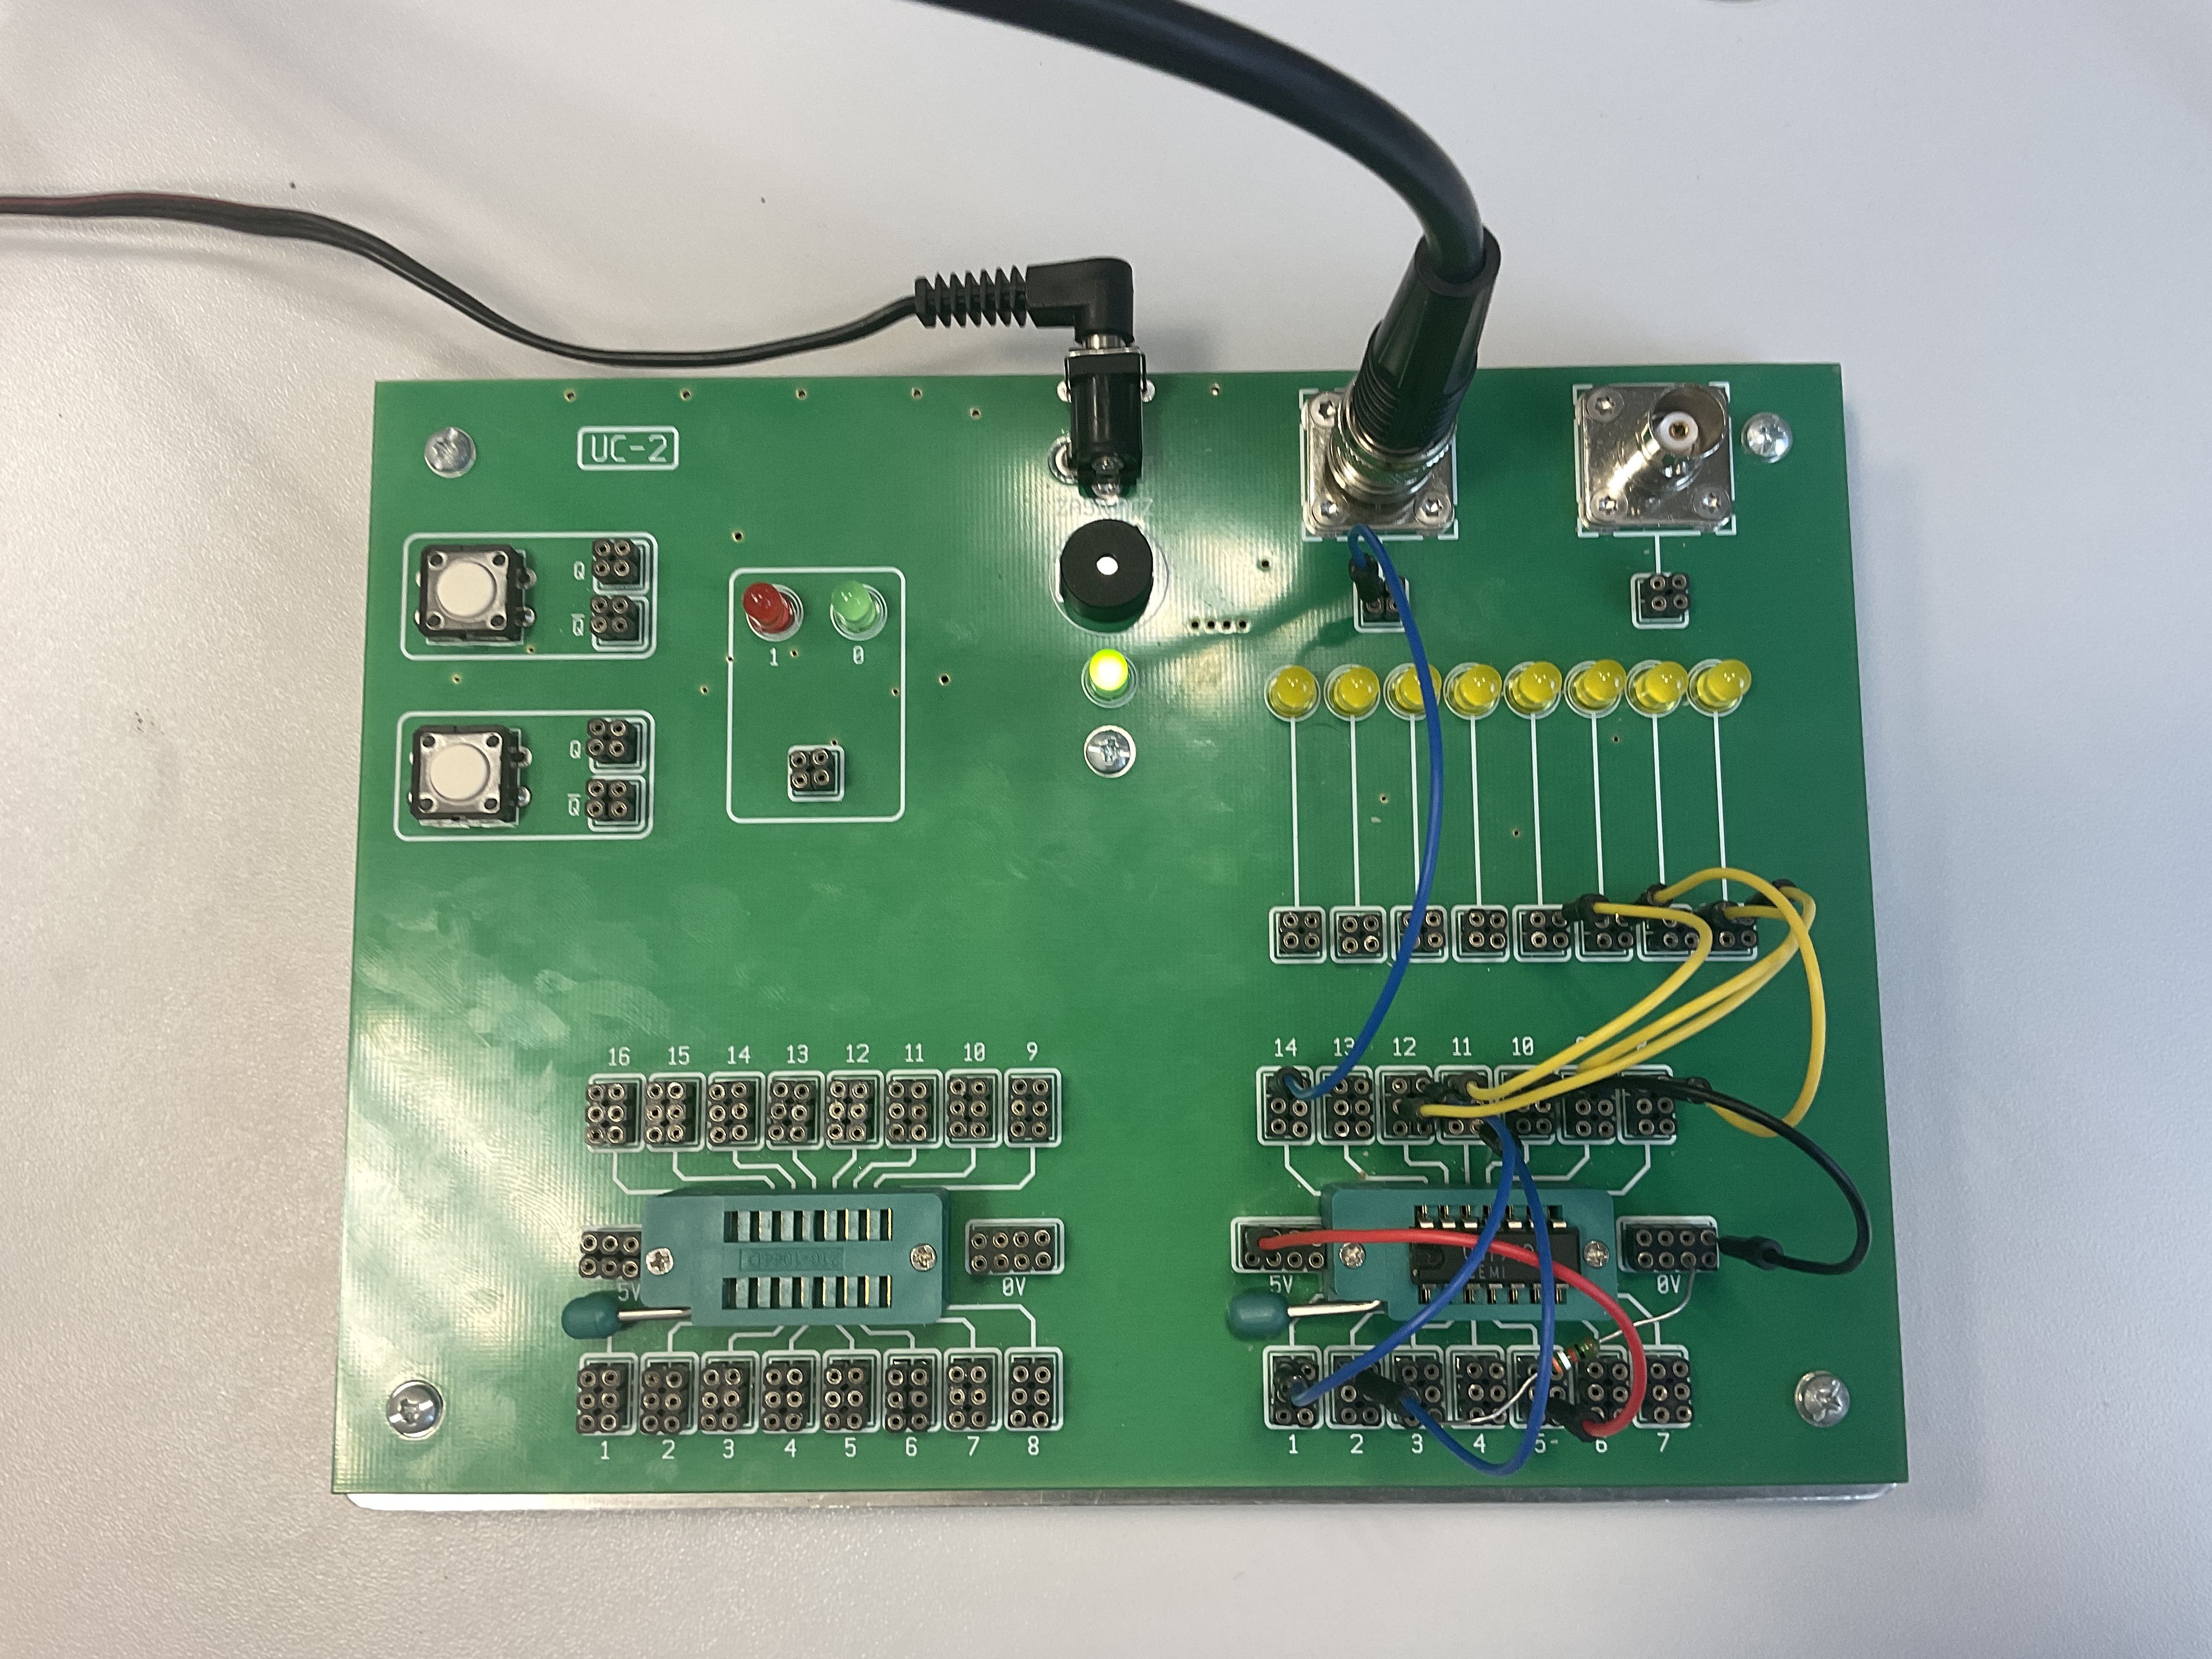
\includegraphics[width=16cm]{C7}
\includegraphics[width=16cm]{A1}
\centering
\captionsetup{labelformat=empty}
\caption{}
\end{figure}

\newpage
\paragraph{Ćwiczenie 5.6 \\}

Zbudowanie licznika modulo 10. \\
	
Moglibyśmy skorzystać ze zbudowanego w poprzednim zadaniu licznika modulo 16 i zerować licznik wtedy, gdy wyjścia przerzutników będą oznaczały stan "10". Licznik osiąga stan 10 kiedy przerzutniki czwarty i drugi (licząc od lewej) mają swoje wyjścia $Q$ ustawione na logiczne 1.  \\

Na nasze szczęście, na układzie scalonym 7493 znajduje się, oprócz 4 przerzutników JK jeszcze jedna bramka NAND. Pozwoli nam ona podać sygnał resetujący (logiczne zero na wejściu RST) do wszystkich czterech przerzutników wtedy, gdy licznik osiągnie stan "10". Nandując wyjścia czwartego i drugiego przerzutnika otrzymamy zero logiczne tylko, jeśli obydwa będą wysokie. \\

Wtedy licznik będzie wyliczał wszystkie liczby od 0 do 9. Schemat takiego układu wygląda następująco:

\begin{center}
\begin{circuitikz} [circuit logic US, scale=1.7]
	
	\ctikzset{multipoles/dipchip/pin spacing=0.5}
	\node [anchor=pin 1, dipchip, num pins=8, hide numbers, no topmark, external pins width=0](jk1) at (0, 0){};
	\node [right, font = \small ] at (jk1.bpin 1) {\textsl{J}};
	\node [right, font = \small ] at (jk1.bpin 2) {\textsl{C}};
	\node [right, font = \small ] at (jk1.bpin 3) {\textsl{R}};
	\node [right, font = \small ] at (jk1.bpin 4) {\textsl{K}};
	\node [left, font = \small ] at (jk1.bpin 8) {\textsl{Q}};

	\node [anchor=pin 1, dipchip, num pins=8, hide numbers, no topmark, external pins width=0](jk2) at (2, 0){};
	\node [right, font = \small ] at (jk2.bpin 1) {\textsl{J}};
	\node [right, font = \small ] at (jk2.bpin 2) {\textsl{C}};
	\node [right, font = \small ] at (jk2.bpin 3) {\textsl{R}};
	\node [right, font = \small ] at (jk2.bpin 4) {\textsl{K}};
	\node [left, font = \small ] at (jk2.bpin 8) {\textsl{Q}};

	\node [anchor=pin 1, dipchip, num pins=8, hide numbers, no topmark, external pins width=0](jk3) at (4, 0){};
	\node [right, font = \small ] at (jk3.bpin 1) {\textsl{J}};
	\node [right, font = \small ] at (jk3.bpin 2) {\textsl{C}};
	\node [right, font = \small ] at (jk3.bpin 3) {\textsl{R}};
	\node [right, font = \small ] at (jk3.bpin 4) {\textsl{K}};
	\node [left, font = \small ] at (jk3.bpin 8) {\textsl{Q}};

	\node [anchor=pin 1, dipchip, num pins=8, hide numbers, no topmark, external pins width=0](jk4) at (6, 0){};
	\node [right, font = \small ] at (jk4.bpin 1) {\textsl{J}};
	\node [right, font = \small ] at (jk4.bpin 2) {\textsl{C}};
	\node [right, font = \small ] at (jk4.bpin 3) {\textsl{R}};
	\node [right, font = \small ] at (jk4.bpin 4) {\textsl{K}};
	\node [left, font = \small ] at (jk4.bpin 8) {\textsl{Q}};

	\draw (jk1.bpin 2) -- node[at end, left]{In} ++(left: 2);

	\draw (jk4.bpin 8) -- node [at end, circle, fill, inner sep=1.3pt](q4){} ++(right: 0.2) -- node[at end, right]{Out} ++(right: 0.6);

	\draw (jk4.bpin 4) -- ++(left: 0.4) -- ++(up: 1.6) -- ++(left: 6.3) to [european resistor] ++(left: 1) -- node[at end, left]{5V} ++(left: 0.2); 
	\draw (jk3.bpin 4) -- ++(left: 0.4) -- node [at end, circle, fill, inner sep=1.3pt]{} ++(up: 1.6); 
	\draw (jk2.bpin 4) -- ++(left: 0.4) -- node [at end, circle, fill, inner sep=1.3pt]{} ++(up: 1.6); 
	\draw (jk1.bpin 4) -- ++(left: 0.4) -- node [at end, circle, fill, inner sep=1.3pt]{} ++(up: 1.6);

	\draw (jk4.bpin 1) -- node [at end, circle, fill, inner sep=1.3pt]{} ++(left: 0.4); 
	\draw (jk3.bpin 1) -- node [at end, circle, fill, inner sep=1.3pt]{} ++(left: 0.4); 
	\draw (jk2.bpin 1) -- node [at end, circle, fill, inner sep=1.3pt]{} ++(left: 0.4); 
	\draw (jk1.bpin 1) -- node [at end, circle, fill, inner sep=1.3pt]{} ++(left: 0.4); 

	\draw (jk2.bpin 2) -- node [at end, circle, fill, inner sep=1.3pt](q1){} ++(left: 0.8) |- (jk1.bpin 8);
	\draw (jk3.bpin 2) -- node [at end, circle, fill, inner sep=1.3pt](q2){} ++(left: 0.8) |- (jk2.bpin 8);
	\draw (jk4.bpin 2) -- node [at end, circle, fill, inner sep=1.3pt](q3){} ++(left: 0.8) |- (jk3.bpin 8);

	\node [rotate=180, nand gate, inputs=nnn] (nand1) at (0, -3.2) {};

	\draw (nand1.input 1) -- node [at end, circle, fill, inner sep=1.3pt]{} ++(right: 6.83);
	\draw (nand1.input 3) -- node [at end, circle, fill, inner sep=1.3pt]{} ++(right: 2.835);

	\draw (jk4.bpin 3) -- ++(left: 0.2) -- ++(down: 1) -- ++(left: 7) |- (nand1.output); 
	\draw (jk3.bpin 3) -- ++(left: 0.2) -- node [at end, circle, fill, inner sep=1.3pt]{} ++(down: 1); 
	\draw (jk2.bpin 3) -- ++(left: 0.2) -- node [at end, circle, fill, inner sep=1.3pt]{} ++(down: 1); 
	\draw (jk1.bpin 3) -- ++(left: 0.2) -- node [at end, circle, fill, inner sep=1.3pt]{} ++(down: 1);

	\draw (q1) -- ++(down: 4) to [empty led] ++(down: 0.5) to [european resistor] ++(down: 1) -- node [ground]{} ++(down: 0.5);
	\draw (q2) -- ++(down: 4) to [empty led] ++(down: 0.5) to [european resistor] ++(down: 1) -- node [ground]{} ++(down: 0.5);;
	\draw (q3) -- ++(down: 4) to [empty led] ++(down: 0.5) to [european resistor] ++(down: 1) -- node [ground]{} ++(down: 0.5);;
	\draw (q4) -- ++(down: 4.4) to [empty led] ++(down: 0.5) to [european resistor] ++(down: 1) -- node [ground]{} ++(down: 0.5);;
\end{circuitikz}
\end{center}

Zbudowałem powyższy układ na płytce UC-2. Zbadałem oscyloskopem przebiegi na wejściu i wyjściu licznika. Filmik z działania licznika załączam w pliku \texttt{Sprawozdanie-cwiczenie5-Jan-Kwinta-Zalacznik3.zip}.

\newpage

\begin{figure}[H]
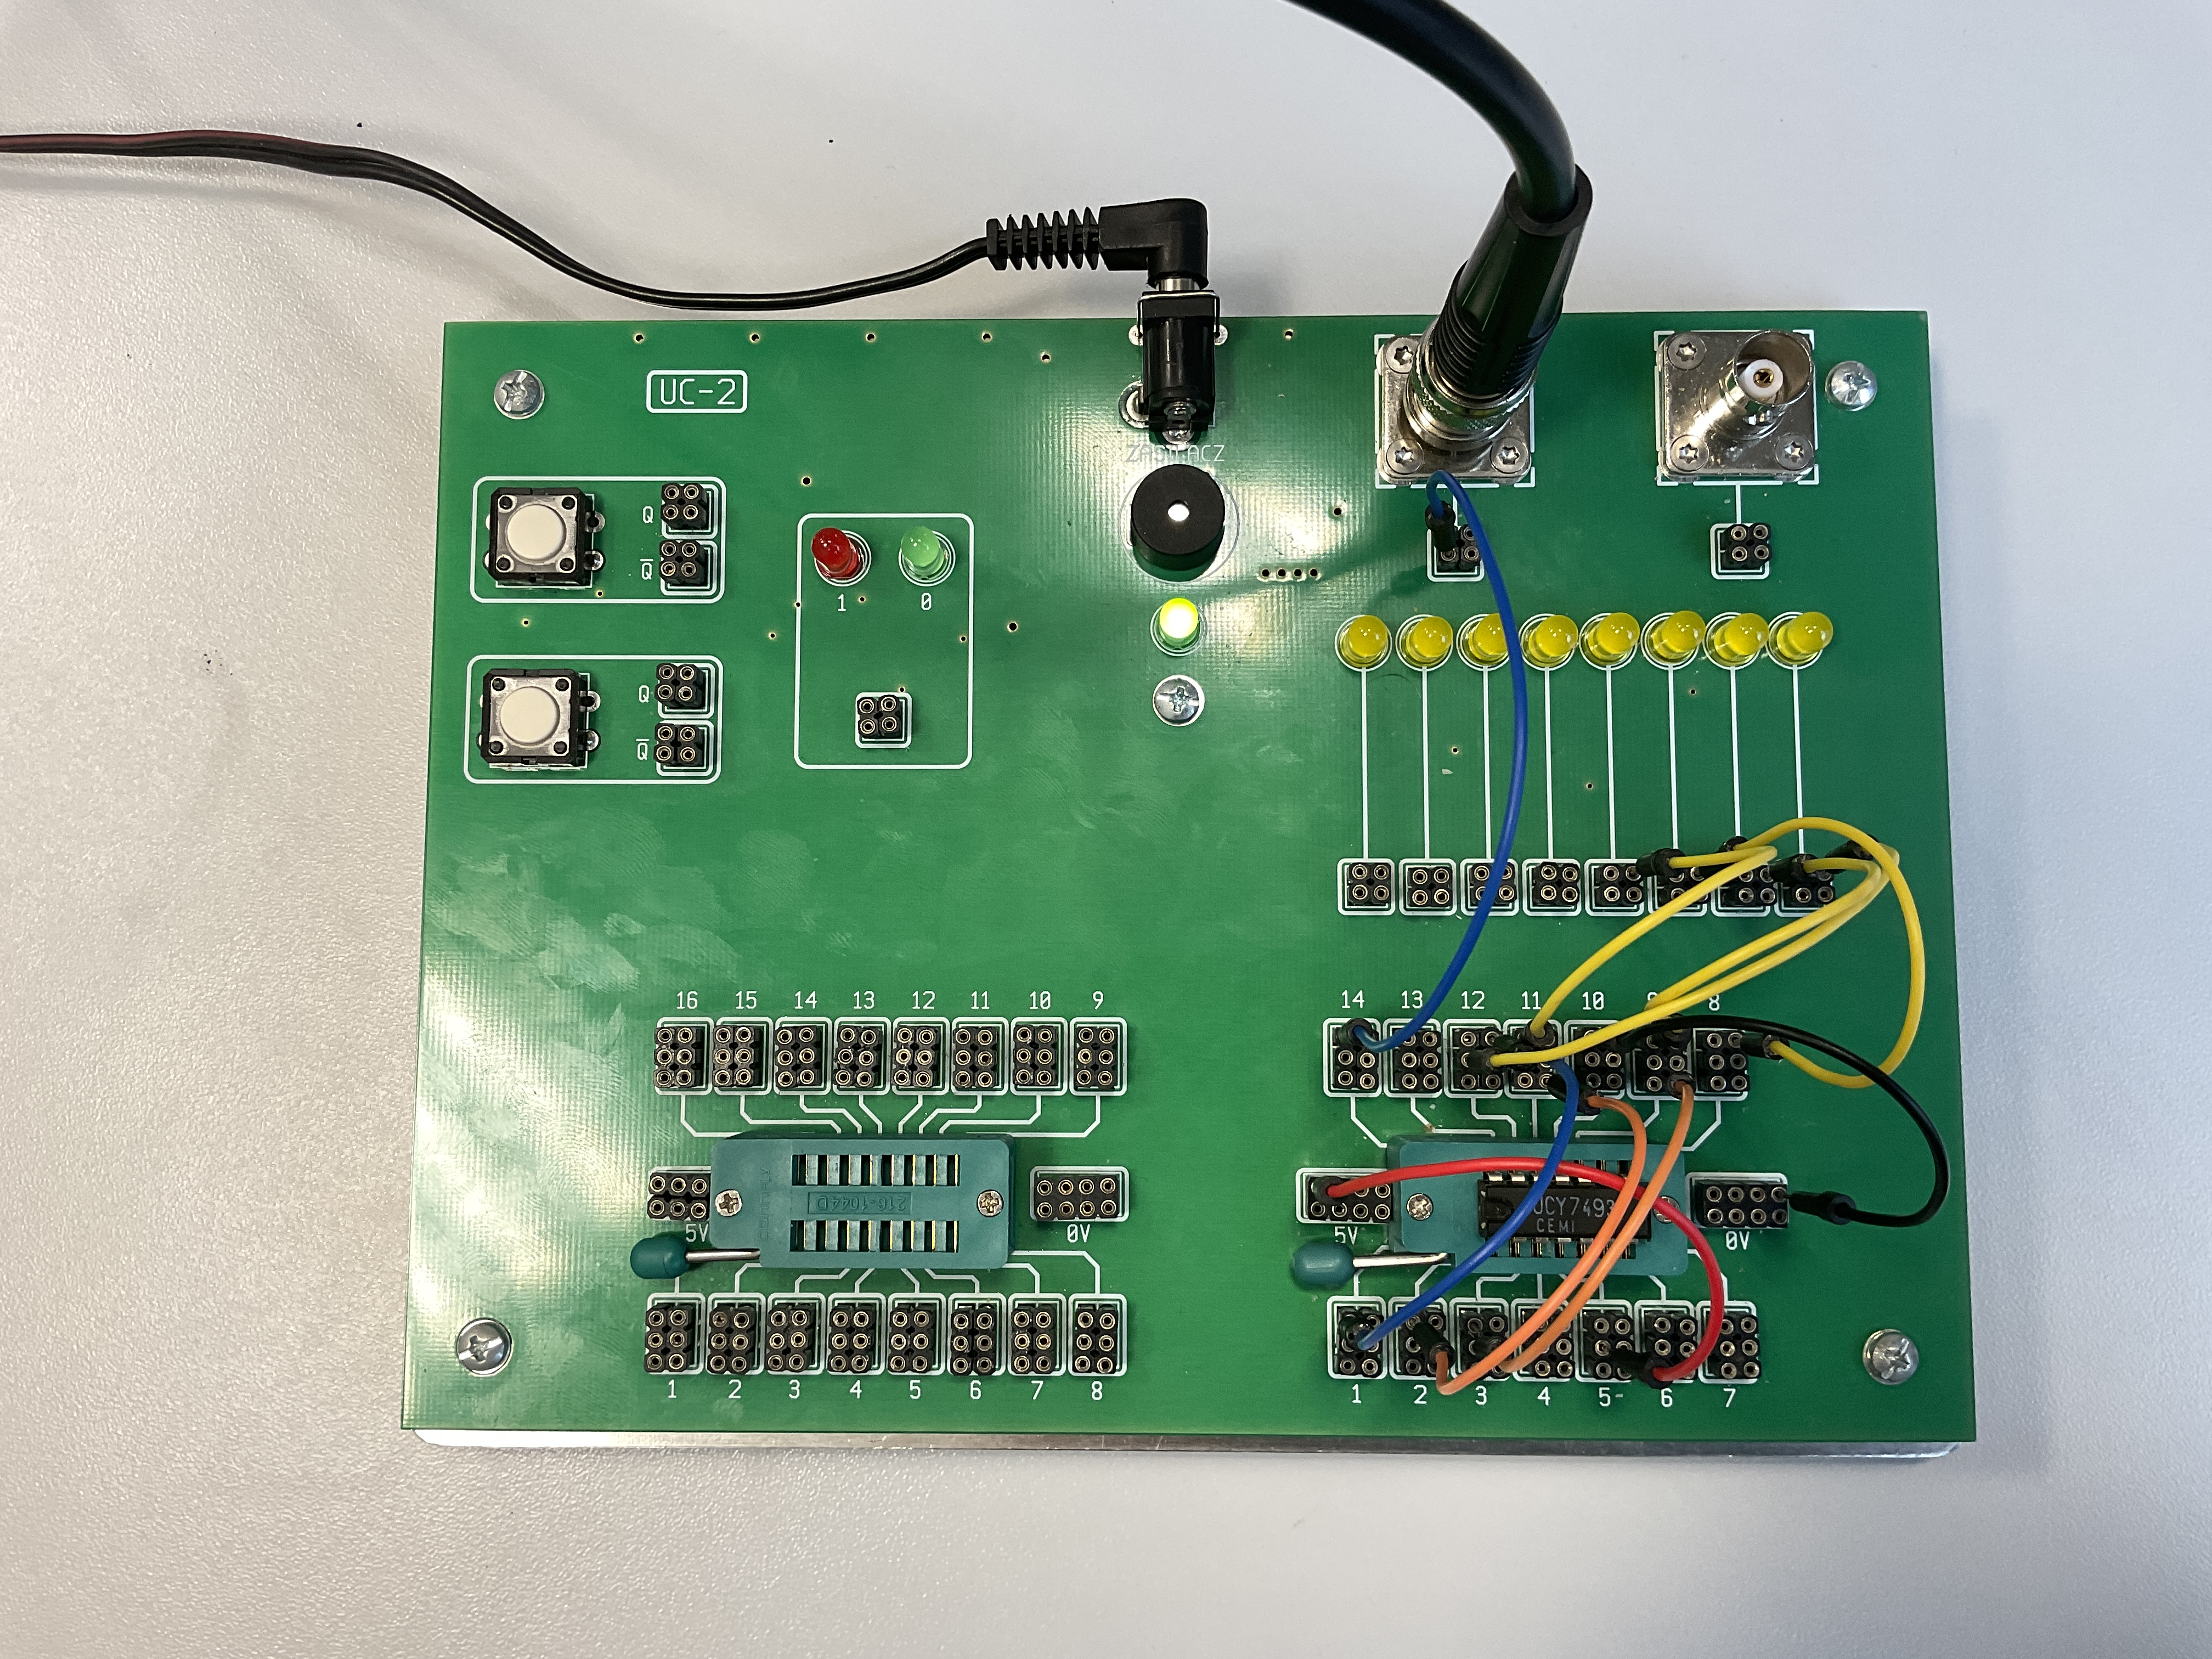
\includegraphics[width=16cm]{C8}
\includegraphics[width=16cm]{A2}
\centering
\captionsetup{labelformat=empty}
\caption{}
\end{figure}

\newpage
\paragraph{Ćwiczenie 5.7 \\}

Sprawdzenie działania rejestrów 74164 i 74165. \\

Układ scalony ośmiobitowego rejestru 74164 ma następujący schemat:

\begin{center}
\begin{circuitikz} [circuit logic US, scale=2]
	
	\ctikzset{multipoles/dipchip/pin spacing=0.5}
	\node [rotate=90, anchor=pin 1, dipchip, num pins=14, hide numbers, scale=2](reg){};

	\node [anchor= south] at (reg.bpin 1) {A};
	\node [anchor= south] at (reg.bpin 2) {B};
	\node [anchor= south] at (reg.bpin 3) {$Q_A$};
	\node [anchor= south] at (reg.bpin 4) {$Q_B$};
	\node [anchor= south] at (reg.bpin 5) {$Q_C$};
	\node [anchor= south] at (reg.bpin 6) {$Q_D$};
	\node [anchor= south] at (reg.bpin 7) {\textsl{GND}};
	\node [anchor= north] at (reg.bpin 8) {\textsl{CLK}};
	\node [anchor= north] at (reg.bpin 9) {\textsl{\ctikztextnot{CLR}}};
	\node [anchor= north] at (reg.bpin 10) {$Q_E$};
	\node [anchor= north] at (reg.bpin 11) {$Q_F$};
	\node [anchor= north] at (reg.bpin 12) {$Q_G$};
	\node [anchor= north] at (reg.bpin 13) {$Q_H$};
	\node [anchor= north] at (reg.bpin 14) {\textsl{Vcc}};

\end{circuitikz}
\end{center}

Rejestr ten posiada 4 wejścia: zegarowe (CLK) i czyszczące (CLR) oraz wejścia danych A i B. Układ posiada także osiem wyjść: $Q_A$, $Q_B$, \ldots $Q_H$, które reprezentują osiem komórek - 8 bitów pamięci rejestru. \\

Z każdym cyklem zegara, podczas zbocza wznoszącego zapisywana jest nowa wartość do komórki A rejestru. Jeżeli na obydwu wejściach A i B podane są logiczne jedynki do komórki A zostaje wpisana jedynka. W przeciwnym wypadku A przyjmuje wartość 0. Wartości pozostałych komórek przesuwane są sekwencyjnie, to znaczy, że przy zboczu wznoszącym zegara komórka H przyjmuje wartość, którą wcześniej miała komórka G, komórka G przyjmuje wartość, którą wcześniej miała komórka F i tak dalej. Z każdym cyklem zegara wartość, która była w komórce H jest tracona. \\

Niezależnie od stanu wejść CLK, A oraz B podanie sygnału niskiego na wejście CLR powoduje wyczyszczenie pamięci, to jest nadanie wszystkim komórkom A, B, \ldots H wartości logicznego zera. \\

Zmontowałem następujący układ: sygnał zegarowy z generatora podałem na wejście CLK układu oraz do próbnika stanów logicznych, by można było widzieć stan zegara. Wyjście $Q$ pierwszego impulsatora podałem na obydwa wejście A i B układu 74164. Wyjście $\overline{Q}$ drugiego impulsatora podałem na wejście CLR rejestru. \\

Za pomocą pierwszego impulsatora jestem w stanie zapisywać bity do pamięci rejestru, a kiedy nacisnę przycisk drugiego impulsatora następuje wyczyszczenie rejestru.

\begin{figure}[H]
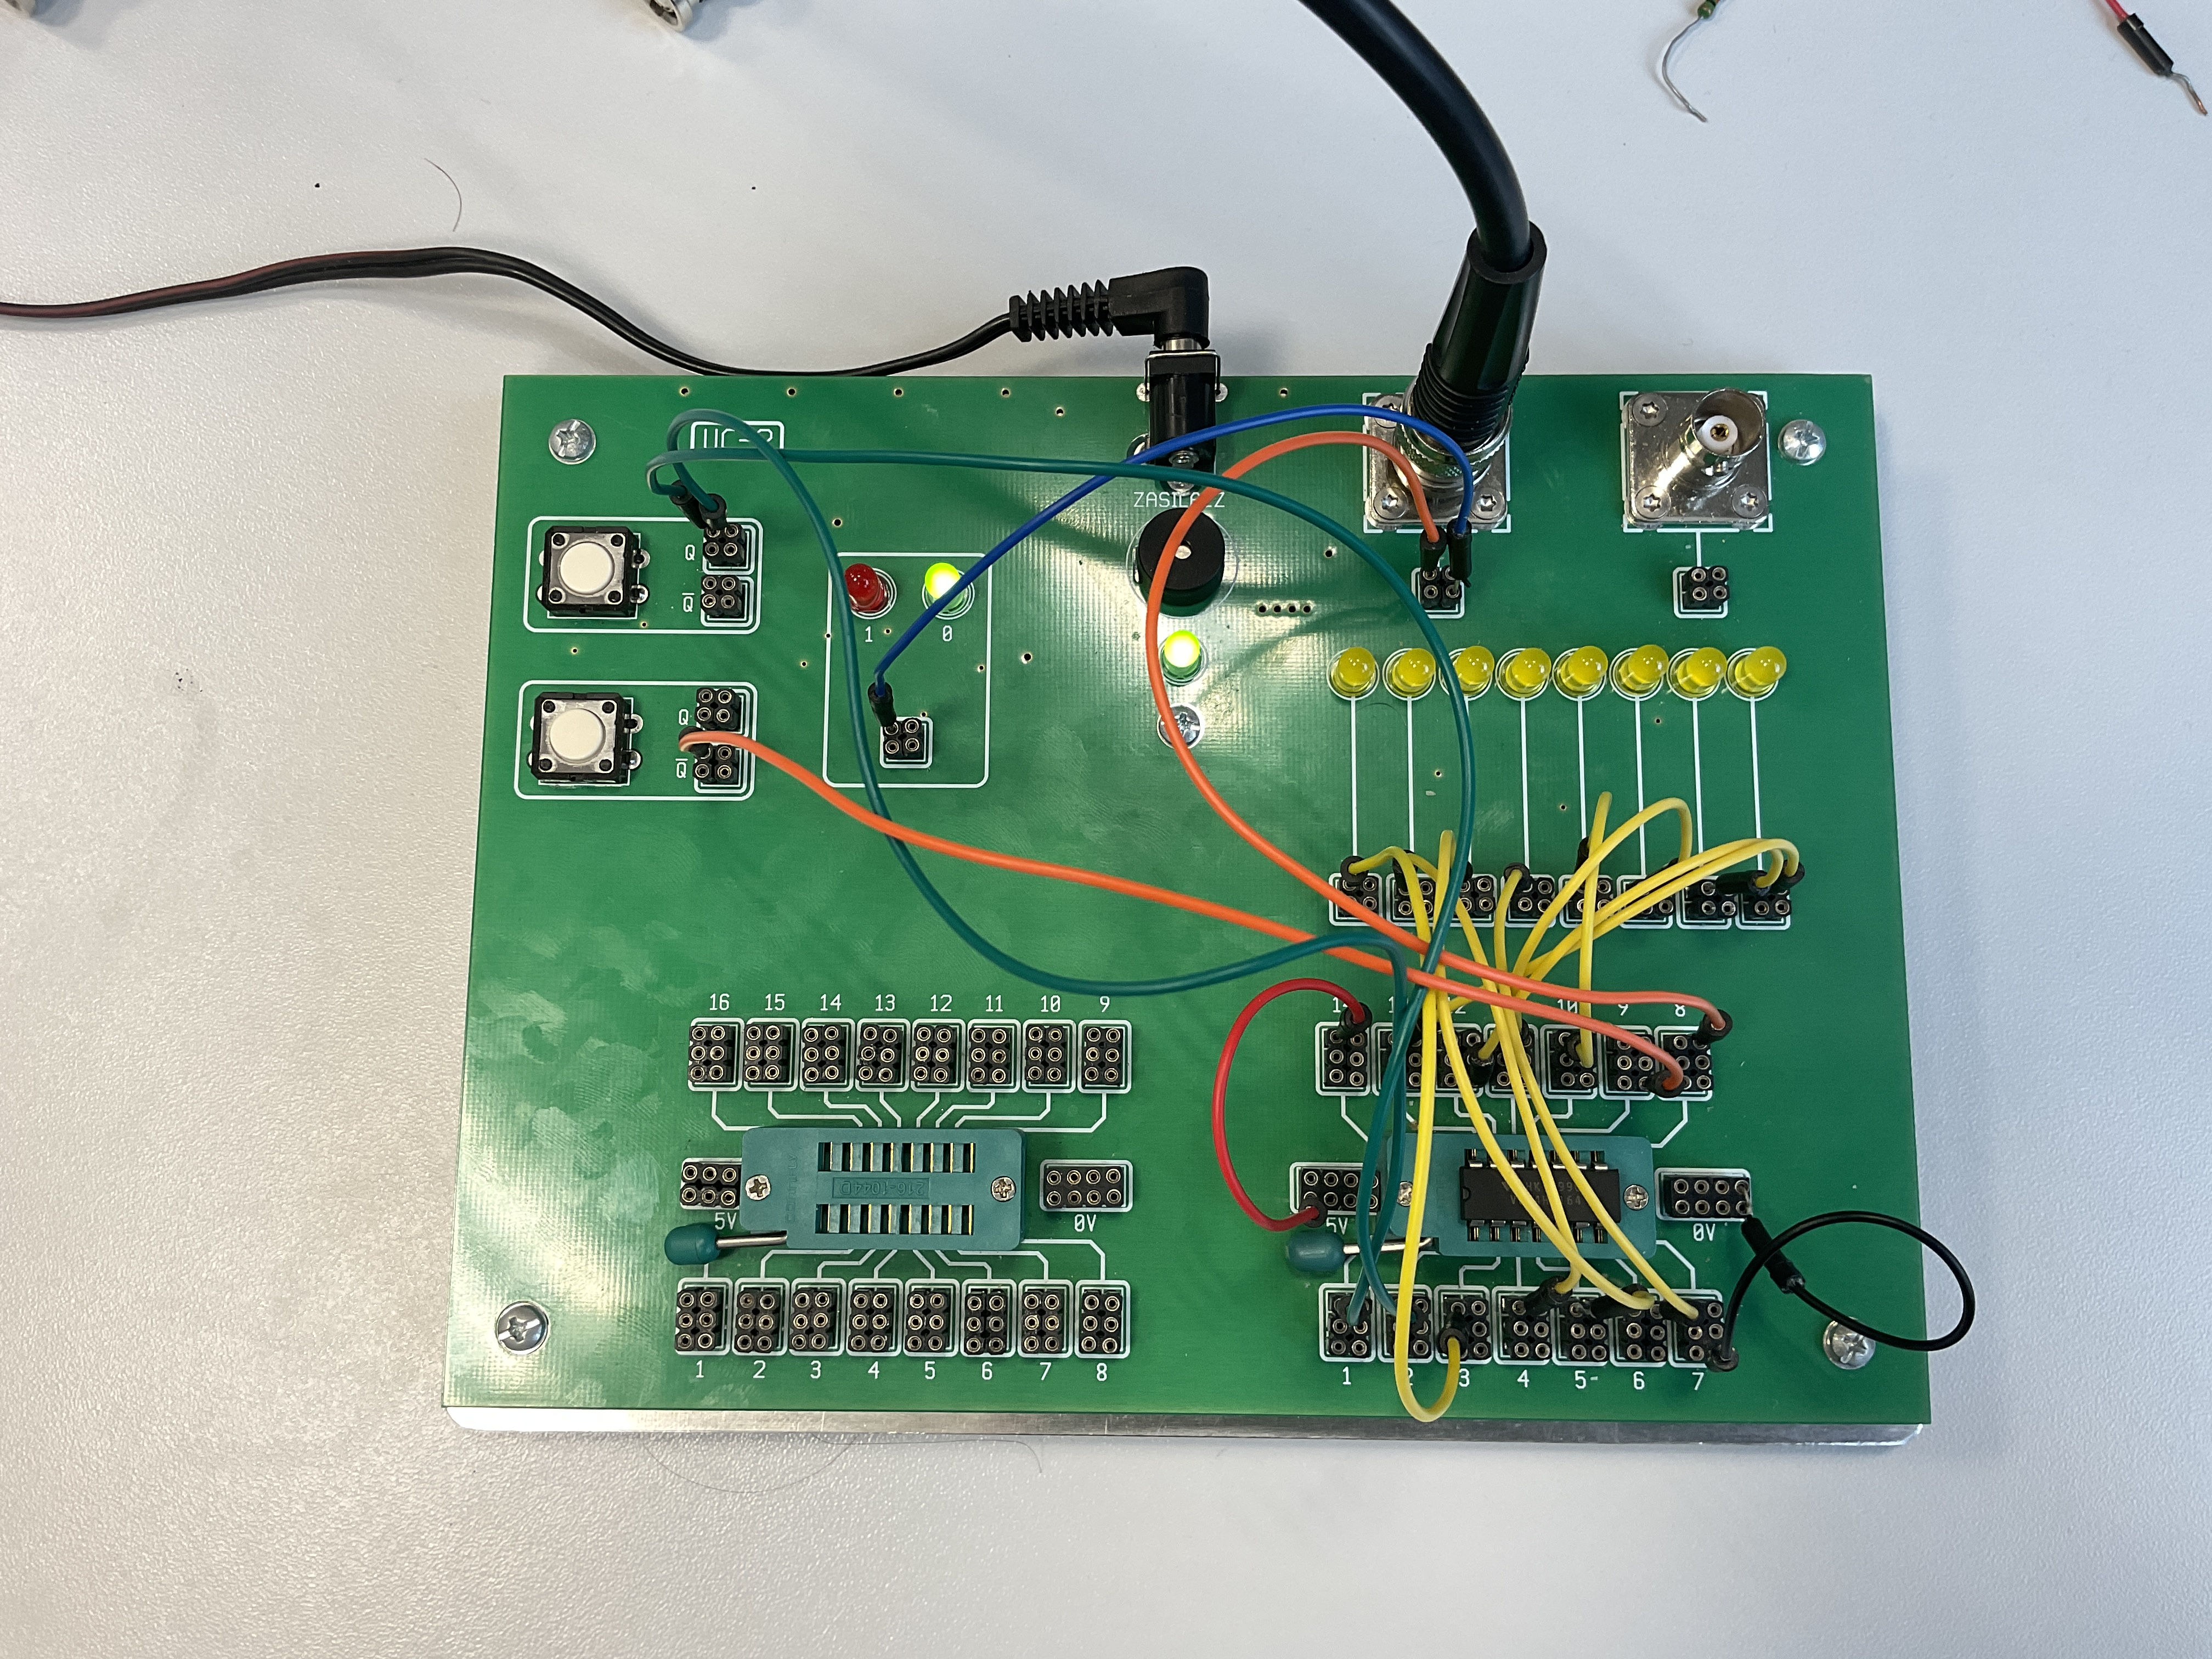
\includegraphics[width=16cm]{C9}
\centering
\captionsetup{labelformat=empty}
\caption{}
\end{figure}

Filmik pokazujący działanie układu zamieszczam w załączniku \\ \texttt{Sprawozdanie-cwiczenie5-Jan-Kwinta-zalacznik4.zip}.

\newpage

Układ scalony ośmiobitowego rejestru 74165 ma następujący schemat:

\begin{center}
\begin{circuitikz} [circuit logic US, scale=2]
	
	\ctikzset{multipoles/dipchip/pin spacing=0.5}
	\node [rotate=90, anchor=pin 1, dipchip, num pins=16, hide numbers, scale=2](reg){};

	\node [anchor= south] at (reg.bpin 1) {\textsl{\ctikztextnot{LD}}};
	\node [anchor= south] at (reg.bpin 2) {CLK};
	\node [anchor= south] at (reg.bpin 3) {E};
	\node [anchor= south] at (reg.bpin 4) {F};
	\node [anchor= south] at (reg.bpin 5) {G};
	\node [anchor= south] at (reg.bpin 6) {H};
	\node [anchor= south] at (reg.bpin 7) {$\overline{Q_H}$};
	\node [anchor= south] at (reg.bpin 8) {\textsl{GND}};
	\node [anchor= north] at (reg.bpin 9) {$Q_H$};
	\node [anchor= north] at (reg.bpin 10) {\textsl{SER}};
	\node [anchor= north] at (reg.bpin 11) {A};
	\node [anchor= north] at (reg.bpin 12) {B};
	\node [anchor= north] at (reg.bpin 13) {C};
	\node [anchor= north] at (reg.bpin 14) {D};
	\node [anchor= north] at (reg.bpin 15) {\textsl{CL IH}};
	\node [anchor= north] at (reg.bpin 16) {\textsl{Vcc}};
\end{circuitikz}
\end{center}

Jest to układ całkiem podobny do poprzedniego. Główną różnicą jest to, że 74165 posiada wejścia szeregowe: oznaczone są jako A, B, \ldots H. W dowolnej chwili pracy rejestru możemy podać na wejścia szeregowe osiem bitów i gdy podamy sygnał niski na wejście \textit{load} (LD) to zostaną one zapisane w pamięci rejestru. \\

Dostępne wyjścia to jedynie wyjście $Q_H$ oraz komplementarne $\overline{Q_H}$. Oznacza to, że w danej chwili widzimy jedynie wierzch stosu pamięci tego układu. Podobnie jak w 74164 bity przesuwają się sekwencyjnie od A do H. W każdym cyklu zegara możemy zapisać nowy bit do komórki A podając go na wejście \textit{serial} (SER). \\

Wejście \textit{clock inhibit} (CL IH) służy do wstrzymywania pracy układu — kiedy zostanie podany na nie sygnał wysoki stan komórek pamięci pozostaje niezmieniany w kolejnych cyklach zegara. \\

Na laboratorium udało mi się podłączyć układ i operować wejściem szeregowym, wejściem blokady zegara (CL IH) i obserwować wyjście $Q_H$. Jednakże, ze względu na małą ilość czasu nie zrealizowałem wpisania 8-bitowego słowa przez wejścia A, B, \ldots H, ani nie połączyłem rejestrów 74164 i 74165 ze sobą. Także ze względu na czas nie udało mi się uwiecznić mojego układu z chipem 74165 na zdjęciach ani na filmiku.

\newpage
\paragraph{Notatki z zeszytu labolatoryjnego \\}
Poniżej załączam notatki z zeszytu laboratoryjnego.

\begin{figure}[H]
\includegraphics[scale=0.2]{B0}
\centering
\captionsetup{labelformat=empty}
\caption{}
\end{figure}

\begin{figure}[H]
\includegraphics[scale=0.2]{B1}
\centering
\captionsetup{labelformat=empty}
\caption{}
\end{figure}

\begin{figure}[H]
\includegraphics[scale=0.2]{B2}
\centering
\captionsetup{labelformat=empty}
\caption{}
\end{figure}

\begin{figure}[H]
\includegraphics[scale=0.2]{B3}
\centering
\captionsetup{labelformat=empty}
\caption{}
\end{figure}



\end{document}
